%%%%%%%%%%%%%%%%%%%%%%%%%%%%%%%%%%%%%%%%%%%%%%%%%%%%%%%%%%%%%%%%%%%%%%%%%%%%
% AGUJournalTemplate.tex: this template file is for articles formatted with LaTeX
%
% This file includes commands and instructions
% given in the order necessary to produce a final output that will
% satisfy AGU requirements, including customized APA reference formatting.
%
% You may copy this file and give it your
% article name, and enter your text.
%
%
% Step 1: Set the \documentclass
%
%

%% To submit your paper:
\documentclass[draft]{agujournal2019}
\usepackage{url} %this package should fix any errors with URLs in refs.
\usepackage{lineno}
\usepackage[inline]{trackchanges} %for better track changes. finalnew option will compile document with changes incorporated.
\usepackage{soul}
\usepackage{amsmath}
\usepackage{listings}
%\usepackage{minted}
\linenumbers

\definecolor{mygreen}{rgb}{0,.5,0}
\definecolor{mygray}{rgb}{0.9,0.9,0.9}

\definecolor{psign}{rgb}{0.9  ,0.1,0.1}
\definecolor{pregime}{rgb}{0.9,0.5,0.0}
\definecolor{pregimet}{rgb}{0.6,0.2,0.2}
\definecolor{pexpo}{rgb}{0.1,0.4,0.7}

\newcommand{\op}{\operatorname}

\lstset{ 
  backgroundcolor=\color{mygray},   % choose the background color; you must add \usepackage{color} or \usepackage{xcolor}; should come as last argument
  basicstyle=\ttfamily,        % the size of the fonts that are used for the code
  breakatwhitespace=false,         % sets if automatic breaks should only happen at whitespace
  breaklines=true,                 % sets automatic line breaking
  captionpos=b,                    % sets the caption-position to bottom
  commentstyle=\color{mygreen},    % comment style
  deletekeywords={...},            % if you want to delete keywords from the given language
  escapeinside={\%*}{*)},          % if you want to add LaTeX within your code
  extendedchars=true,              % lets you use non-ASCII characters; for 8-bits encodings only, does not work with UTF-8
  frame=single,	                   % adds a frame around the code
  keepspaces=true,                 % keeps spaces in text, useful for keeping indentation of code (possibly needs columns=flexible)
  keywordstyle=\color{mygreen}\textbf,       % keyword style
  language=Matlab,                 % the language of the code
  morekeywords={julia},            % if you want to add more keywords to the set
  numbers=left,                    % where to put the line-numbers; possible values are (none, left, right)
  numbersep=5pt,                   % how far the line-numbers are from the code
  numberstyle=\tiny\color{gray}, % the style that is used for the line-numbers
  rulecolor=\color{black},         % if not set, the frame-color may be changed on line-breaks within not-black text (e.g. comments (green here))
  showspaces=false,                % show spaces everywhere adding particular underscores; it overrides 'showstringspaces'
  showstringspaces=false,          % underline spaces within strings only
  showtabs=false,                  % show tabs within strings adding particular underscores
  stepnumber=1,                    % the step between two line-numbers. If it's 1, each line will be numbered
  stringstyle=\color{black},     % string literal style
  tabsize=2,	                   % sets default tabsize to 2 spaces
  title=\lstname                   % show the filename of files included with \lstinputlisting; also try caption instead of title
}

\newcommand*\patchAmsMathEnvironmentForLineno[1]{%
  \expandafter\let\csname old#1\expandafter\endcsname\csname #1\endcsname
  \expandafter\let\csname oldend#1\expandafter\endcsname\csname end#1\endcsname
  \renewenvironment{#1}%
     {\linenomath\csname old#1\endcsname}%
     {\csname oldend#1\endcsname\endlinenomath}}% 
\newcommand*\patchBothAmsMathEnvironmentsForLineno[1]{%
  \patchAmsMathEnvironmentForLineno{#1}%
  \patchAmsMathEnvironmentForLineno{#1*}}%
\AtBeginDocument{%
\patchBothAmsMathEnvironmentsForLineno{equation}%
\patchBothAmsMathEnvironmentsForLineno{align}%
\patchBothAmsMathEnvironmentsForLineno{flalign}%
\patchBothAmsMathEnvironmentsForLineno{alignat}%
\patchBothAmsMathEnvironmentsForLineno{gather}%
\patchBothAmsMathEnvironmentsForLineno{multline}%
}

%%%%%%%
% As of 2018 we recommend use of the TrackChanges package to mark revisions.
% The trackchanges package adds five new LaTeX commands:
%
%  \note[editor]{The note}
%  \annote[editor]{Text to annotate}{The note}
%  \add[editor]{Text to add}
%  \remove[editor]{Text to remove}
%  \change[editor]{Text to remove}{Text to add}
%
% complete documentation is here: http://trackchanges.sourceforge.net/
%%%%%%%

\draftfalse

%% Enter journal name below.
%% Choose from this list of Journals:
%
% JGR: Atmospheres
% JGR: Biogeosciences
% JGR: Earth Surface
% JGR: Oceans
% JGR: Planets
% JGR: Solid Earth
% JGR: Space Physics
% Global Biogeochemical Cycles
% Geophysical Research Letters
% Paleoceanography and Paleoclimatology
% Radio Science
% Reviews of Geophysics
% Tectonics
% Space Weather
% Water Resources Research
% Geochemistry, Geophysics, Geosystems
% Journal of Advances in Modeling Earth Systems (JAMES)
% Earth's Future
% Earth and Space Science
% Geohealth
%
% ie, \journalname{Water Resources Research}

\journalname{Journal of Advances in Modeling Earth Systems}


\begin{document}

%% ------------------------------------------------------------------------ %%
%  Title
%
% (A title should be specific, informative, and brief. Use
% abbreviations only if they are defined in the abstract. Titles that
% start with general keywords then specific terms are optimized in
% searches)
%
%% ------------------------------------------------------------------------ %%

% Example: \title{This is a test title}

\title{Weather and climate models in 16bit: Posit, floating-point or mixed precision arithmetic?}

%% ------------------------------------------------------------------------ %%
%
%  AUTHORS AND AFFILIATIONS
%
%% ------------------------------------------------------------------------ %%

% Authors are individuals who have significantly contributed to the
% research and preparation of the article. Group authors are allowed, if
% each author in the group is separately identified in an appendix.)

% List authors by first name or initial followed by last name and
% separated by commas. Use \affil{} to number affiliations, and
% \thanks{} for author notes.
% Additional author notes should be indicated with \thanks{} (for
% example, for current addresses).

% Example: \authors{A. B. Author\affil{1}\thanks{Current address, Antartica}, B. C. Author\affil{2,3}, and D. E.
% Author\affil{3,4}\thanks{Also funded by Monsanto.}}

\authors{M. Kl\"{o}wer\affil{1}, P. D. D\"{u}ben\affil{2}, and T. N. Palmer\affil{1}}


% \affiliation{1}{First Affiliation}
% \affiliation{2}{Second Affiliation}
% \affiliation{3}{Third Affiliation}
% \affiliation{4}{Fourth Affiliation}

\affiliation{1}{Atmospheric, Oceanic and Planetary Physics, University of Oxford, Oxford, UK}
\affiliation{2}{European Centre for Medium-Range Weather Forecasts, Reading, UK}
%(repeat as many times as is necessary)

%% Corresponding Author:
% Corresponding author mailing address and e-mail address:

% (include name and email addresses of the corresponding author.  More
% than one corresponding author is allowed in this LaTeX file and for
% publication; but only one corresponding author is allowed in our
% editorial system.)

% Example: \correspondingauthor{First and Last Name}{email@address.edu}

\correspondingauthor{M. Kl\"{o}wer}{milan.kloewer@physics.ox.ac.uk}

%% Keypoints, final entry on title page.

%  List up to three key points (at least one is required)
%  Key Points summarize the main points and conclusions of the article
%  Each must be 140 characters or fewer with no special characters or punctuation and must be complete sentences

% Example:
% \begin{keypoints}
% \item	List up to three key points (at least one is required)
% \item	Key Points summarize the main points and conclusions of the article
% \item	Each must be 140 characters or fewer with no special characters or punctuation and must be complete sentences
% \end{keypoints}

\begin{keypoints}
\item $\circ$ Posit numbers have smaller rounding errors compared to floating-point numbers in weather and climate applications, enabling reliable shallow water simulations entirely computed with 16bit arithmetic.

\item $\circ$ Errors caused by 16bit floating-point arithmetic are strongly reduced with key computations in 32bit, which can be implemented on present-day hardware.

\item $\circ$ 16 or even 8bit communication of boundary values, preferably encoded as posit numbers, introduces negligible errors, providing perspectives for reduced data communication for weather and climate models computed in parallel.

\end{keypoints}

%% ------------------------------------------------------------------------ %%
%
%  ABSTRACT and PLAIN LANGUAGE SUMMARY
%
% A good Abstract will begin with a short description of the problem
% being addressed, briefly describe the new data or analyses, then
% briefly states the main conclusion(s) and how they are supported and
% uncertainties.

% The Plain Language Summary should be written for a broad audience,
% including journalists and the science-interested public, that will not have 
% a background in your field.
%
% A Plain Language Summary is required in GRL, JGR: Planets, JGR: Biogeosciences,
% JGR: Oceans, G-Cubed, Reviews of Geophysics, and JAMES.
% see http://sharingscience.agu.org/creating-plain-language-summary/)
%
%% ------------------------------------------------------------------------ %%

%% \begin{abstract} starts the second page

\begin{abstract}
Posit numbers, a recently proposed alternative to floating-point numbers, claim to have smaller arithmetic rounding errors in many applications. By studying weather and climate models of low and medium complexity (the Lorenz system and a shallow water model) we present benefits of posits compared to floats at 16bit. As a standardized posit processor does not exist yet, we emulate posit arithmetic on a conventional processor. Forecasts based on posits are clearly more accurate than floats in shallow water simulations. Even the rounding error of 16bit floats is not larger than the discretization error, that results from simulations run at half the spatial resolution. No 16bit format was found to have a significant impact on the climatological mean state, however, the variability increased up to 30\%. Instabilities in the flow field, triggered by rounding errors of 16bit formats, were found to not alter the dynamics of the simulated flow significantly. Mixing 16bit arithmetic with 32bit for key computations strongly reduces errors and is promising for present-day float-based hardware. Reduced precision communication of boundary values with 16 or 8bit encoded as floats or posits introduces negligible errors, presenting a perspective for reduced data communication within a computer cluster. The results promote the potential of 16bit formats for parts of complex weather and climate models, for which rounding errors would be masked by intitial condition, model or discretization error.
\end{abstract}

%% ------------------------------------------------------------------------ %%
%
%  TEXT
%
%% ------------------------------------------------------------------------ %%

\section{Introduction}
\label{sec:intro}

Weather and climate models provide predictions that are of great importance for society and economy. The Earth's climate system remains very difficult to predict even with the computational resources of the world's largest supercomputers, due to its complexity and non-linear dynamics that couple all features from the smallest time and length-scales to the largest. The forecast error of a weather forecast model has several origins \cite{Palmer2012a,Palmer2015}: (i) Initial and boundary condition errors, which result from observations, data assimilation and external factors; (ii) model error, i.e. the difference between the mathematical model and the real world; (iii) discretisation error resulting from a finite spatial and temporal resolution of the discretised equations and (iv) rounding errors with finite precision arithmetic. In general, the forecast error is dominated by (i-iii), depending on the forecast variable and the forecast lead time. In contrast, rounding errors are usually negligible with the IEEE 754 standard on 64 bit double precision floating-point numbers \cite{IEEE}, which is still the standard for the majority of operational weather forecasts and in climate models.

Research on reduced precision floating-point arithmetics is motivated by the potential for faster processing and communication between different elements of the computing architecture. The gained speed can be traded for increased complexity of simulations, resulting in more accurate predictions of weather and climate. The Integrated Forecast System at the European Centre for Medium-Range Weather Forecasts can be run almost entirely at single precision (32 bit) without a decrease in forecast skill \cite{Vana2017} but in 60\% of the run-time. Similar progress was made at MeteoSwiss with their weather forecast model COSMO \cite{Rudisuhli2013}. 

The recent boom of deep learning techniques, that require low numerical precision but high computational performance, will influence hardware development to offer more flexibility for the use of reduced numerical precision. Using simplistic chaotic models, it was shown that the majority of 64 bits at double precision do not contain real information \cite{Jeffress2017}. Running algorithms used for weather forecast models at precision lower than single, for example with half precision 16-bit floats, is an active field of research, but remains challenging \cite{Duben2014,Thornes2017,Hatfield2018,Duben2018}. Most research on reduced precision modelling for weather and climate applications makes use of software emulators \cite{Dawson2017} that provide other arithmetics than the widely supported single and double precision floats. This comes with the disadvantage that simulations are orders of magnitude slower. However, software emulation allows a scientific evaluation of the use of reduced numerical precision for weather and climate simulations with no need to port the models to special hardware (such as FPGAs, \cite{Russell2017}).
 
Posit numbers are a recently proposed alternative to floats and claim to provide more precision in arithmetic calculations with fewer bits in algorithms of linear algebra or machine learning \cite{Gustafson2017}. However, posits remain untested for weather and climate simulations. This study therefore focuses on posit arithmetic as an alternative to floating-point arithmetic at the appealing size of 16 bit for weather and climate models. We use a Julia-based emulator on a conventional CPU, as posit hardware is not yet available. Posit research currently focuses on hardware implementations \cite{VanDam2018,Chen2018,Chaurasiya2018,Glaser2017}.

The study  is structured as follows: Section \ref{sec:posits} introduces the posit number format and the concept of decimal precision. We analyse the dynamics of a chaotic model at low complexity with posit arithmetic using the Lorenz 1963 system in section \ref{sec:L63}. In section \ref{sec:swm} we evaluate posit arithmetic in the shallow water equations, a two dimensional fluid circulation model. Section \ref{sec:discuss} discusses the results and summarises the conclusions.

\section{Posit numbers}
\label{sec:posits}
\subsection{The posit number format}
\label{sec:posit_methods}

The IEEE standard on floating-point arithmetic \cite{IEEE} defines how floats encode a real number in terms of a sign bit, and a fixed number of exponent and significant bits (16bit half precision floats have 1 sign, 5 exponent and 10 significant bits). Consequently, they have a constant number of significant digits throughout their range of representable numbers. This is in contrast to posit numbers, which extend floating-point arithmetic by introducing regime bits, which are mostly responsible for the dynamic range of representable numbers. Instead of having a fixed length, regime bits are defined as the sequence of identical bits after the sign bit, which are eventually terminated by an opposite bit. The flexible length allows the significand (or mantissa) to occupy more bits when less regime bits are needed, which is the case for numbers around one. A resulting higher precision around one is traded against a gradually lower precision for very large or very small numbers. A positive posit number $p$ is decoded as \cite{Gustafson2017,Gustafson2017b} (negative posit numbers are converted first to their two's complement, see Eq. \ref{eq:2comp})
\begin{equation}
p = (-1)^{sign~bit} \cdot useed^k \cdot 2^e \cdot (1+f)
\label{eq:posit}
\end{equation}
where $k$ is the number of regime bits. $e$ is the integer represented by the exponent bits and $f$ is the fraction which is encoded in the fraction (or significant) bits. The base $useed = 2^{2^{e_s}}$ is determined by the number of exponent bits $e_s$. More exponent bits increase - by increasing $useed$ - the dynamic range of representable numbers for the cost of precision. The exponent bits themselves do not affect the dynamic range by changing the value of $2^e$ in Eq. \ref{eq:posit}. They fill gaps of powers of 2 spanned by $useed = 4,16,256,...$ for $e_s=1,2,3,...$, and every posit number can be written as $p = \pm 2^n \cdot (1+f)$ with a given integer $n$ \cite{Gustafson2017,Chen2018}. We will use a notation where Posit($n$,$e_s$) defines the posit numbers with $n$ bits including $e_s$ exponent bits. A posit example is provided in the Posit(8,1)-system (i.e. $useed = 4$)
\begin{equation}
57 \approx {\color{psign}0}{\color{pregime}111}{\color{pregimet}0}{\color{pexpo}1}11_{\op{Posit}(8,1)} = (-1)^{\color{psign}0} \cdot 4^{\color{pregime}2} \cdot 2^{\color{pexpo}1} \cdot (1+2^{-1}+2^{-2}) = 56
\label{eq:posit_pos}
\end{equation}
The sign bit is given in red, regime bits in orange, the terminating regime bit in brown, the exponent bit in blue and the fraction bits in black. The $k$-value is inferred from the number of regime bits, that are counted as negative for the bits being 0, and positive, but subtract 1, for the bits being 1. The exponent bits are interpreted as unsigned integer and the fraction bits follow the IEEE floating-point standard for significant bits. For negative numbers, i.e. the sign bit being 1, all other bits are first converted to their two's complement (denoted with an underscore subscript) by flipping all bits and adding 1,
\begin{equation}
\begin{split}
-0.28 &  \approx 11011110_{\op{Posit}(8,1)} = {\color{psign}1}{\color{pregime}0}{\color{pregimet}1}{\color{pexpo}0}0010\_ \\
& = (-1)^{\color{psign}1} \cdot 4^{\color{pregime}-1} \cdot 2^{\color{pexpo}0} \cdot (1+2^{-3}) = -0.28125.
\end{split}
\label{eq:2comp}
\end{equation}
After the conversion to the two's complement, the bits are interpreted in the same way as in Eq. \ref{eq:posit_pos}.

Posits also come with a no overflow/no underflow-rounding mode: Where floats overflow and return infinity when the exact result of an arithmetic operation is larger than the largest representable number ($maxpos$), posit arithmetic returns $maxpos$ instead, and similarly for underflow where the smallest representable number $minpos$ is returned. This is motivated as rounding to infinity returns a result that is infinitely less correct than $maxpos$, although often desired to indicate that an overflow occurred in the simulation. Instead, it is proposed to perform overflow-like checks on the software level to simplify exception handling on hardware \cite{Gustafson2017b}.

The posit number framework also highly recommends \emph{quires}, an additional register on hardware to store intermediate results. Fused operations like \emph{multiply-add} can therefore be executed with a single rounding error without the rounding of intermediate results. The quire concept could also be applied to floating-point arithmetic, but is technically difficult to implement on hardware as the required registers would need to be much larger in size. For fair comparison we do not take quires into account. The posit number format is explained in more detail in \citeA{Gustafson2017b}.

\subsection{Emulating posit numbers in the Julia language}
\label{sec:Julia}

In order to use posits on a conventional CPU we developed the posit emulator \emph{SoftPosit.jl} \cite{Kloewer2019}, a wrapper for the C-based library SoftPosit \cite{Heung2019}, written in Julia \cite{Bezanson2014}. This emulator defines conversion and arithmetic operations with posits. Julia's programming paradigms around \emph{multiple dispatch} and \emph{type stability} facilitate the use of arbitrary number formats without the need to rewrite an algorithm. As this is an essential feature of the Julia language and extensively made use of in this study, we briefly outline the benefits of Julia by computing the harmonic sum with various number types as an example.

\begin{figure}[htbp]
%\begin{minted}[breaklines,escapeinside=||,mathescape=true,baselinestretch=0.7, linenos, numbersep=3pt, bgcolor=mygray,gobble=2, frame=lines, fontsize=\small, framesep=2mm]{julia} 
%  function harmonic_sum(::Type{T},steps::Int=2000) where T
%
%      s = zero(T)
%      o = one(T)
%
%      for i in 1:steps
%
%          s_old = s
%          s += o/T(i)
%
%          if s == s_old    # check for convergence
%              println(Float64(s),i)
%              break
%         end
%      end
%  end
%\end{minted}
\caption{A type-flexible harmonic sum function in the Julia language.}
\label{fig:emulator}
\end{figure}

Executing the function \texttt{harmonic\_sum} for the first time with a type \texttt{T} as the first argument, triggers Julia's \emph{just-in-time} compiler. The function is type stable, as the types of all variables are declared. At the same time Julia allows for type flexibility, as its \emph{multiple dispatch} means that calling  \texttt{harmonic\_sum} with another type \texttt{T2} will result in a separately compiled function for \texttt{T2}. We can therefore compute the harmonic sum with aribitrary number types, as long as the zero-element \texttt{zero(T)}; the one-element \texttt{one(T)}; addition; division; conversion from integer and conversion to float are defined for \texttt{T}. 

\begin{figure}[htbp]
%\begin{minted}[breaklines,escapeinside=||,mathescape=true,baselinestretch=0.7, linenos, numbersep=3pt, bgcolor=mygray, gobble=2, frame=lines, fontsize=\small, framesep=2mm]{julia} 
%julia> using SoftPosit
%julia> using BFloat16s
%julia> harmonic_sum(Float16)
%(7.0859375, 513)
%julia> harmonic_sum(BFloat16)
%(5.0625, 65)
%julia> harmonic_sum(Posit16)
%(7.77734375, 1024)
%\end{minted}
\caption{Harmonic sum example use of the posit emulator \emph{SoftPosit.jl} in the Julia shell. \texttt{Posit16} is the Posit(16,1) standard.}
\label{fig:emulator}
\end{figure}

The harmonic sum converges after 513 elements when using Float16. The precision of BFloat16 is so low that the sum already converges after 65 elements, as the addition of the next term $1/66$ is round back to 5.0625. We identify the addition of small terms to prognostic variables of size $\mathcal{O}(1)$ as one of the major challenges with low precision arithmetic, which is discussed in more detail in section \ref{sec:mixed}. Using 16bit posits with 1 exponent bit, the sum only converges after 1024 terms, due to the higher decimal precision of posits around 1. 

We implement this type-flexible programming paradigm in the numerical integration of the Lorenz equations (section \ref{sec:L63}) and the shallow water model (section \ref{sec:swm}), which allows various number types to be used interchangeably.

\subsection{Decimal precision}
\label{sec:decprec}

The decimal precision is defined as \cite{Gustafson2017,Gustafson2017b}
\begin{equation}
\op{decimal} \op{precision} = -\log_{10} \vert \log_{10}( \frac{x_\text{repr}}{x_\text{exact}} ) \vert
\end{equation}
where $x_\text{exact}$ is the exact result of an arithmetic operation and $x_\text{repr}$ is the representable number that $x_\text{exact}$ is rounded to, given a specified rounding mode. For round-to-nearest rounding mode, the decimal precision approaches infinity when the exact result approaches the representable number and has a minimum in between two representable numbers. This minimum defines the \emph{worst-case} decimal precision, i.e. the decimal precision when the rounding error is maximised. The worst-case decimal precision is the number of decimal places that are at least correct after rounding. 

\begin{figure}[htbp]
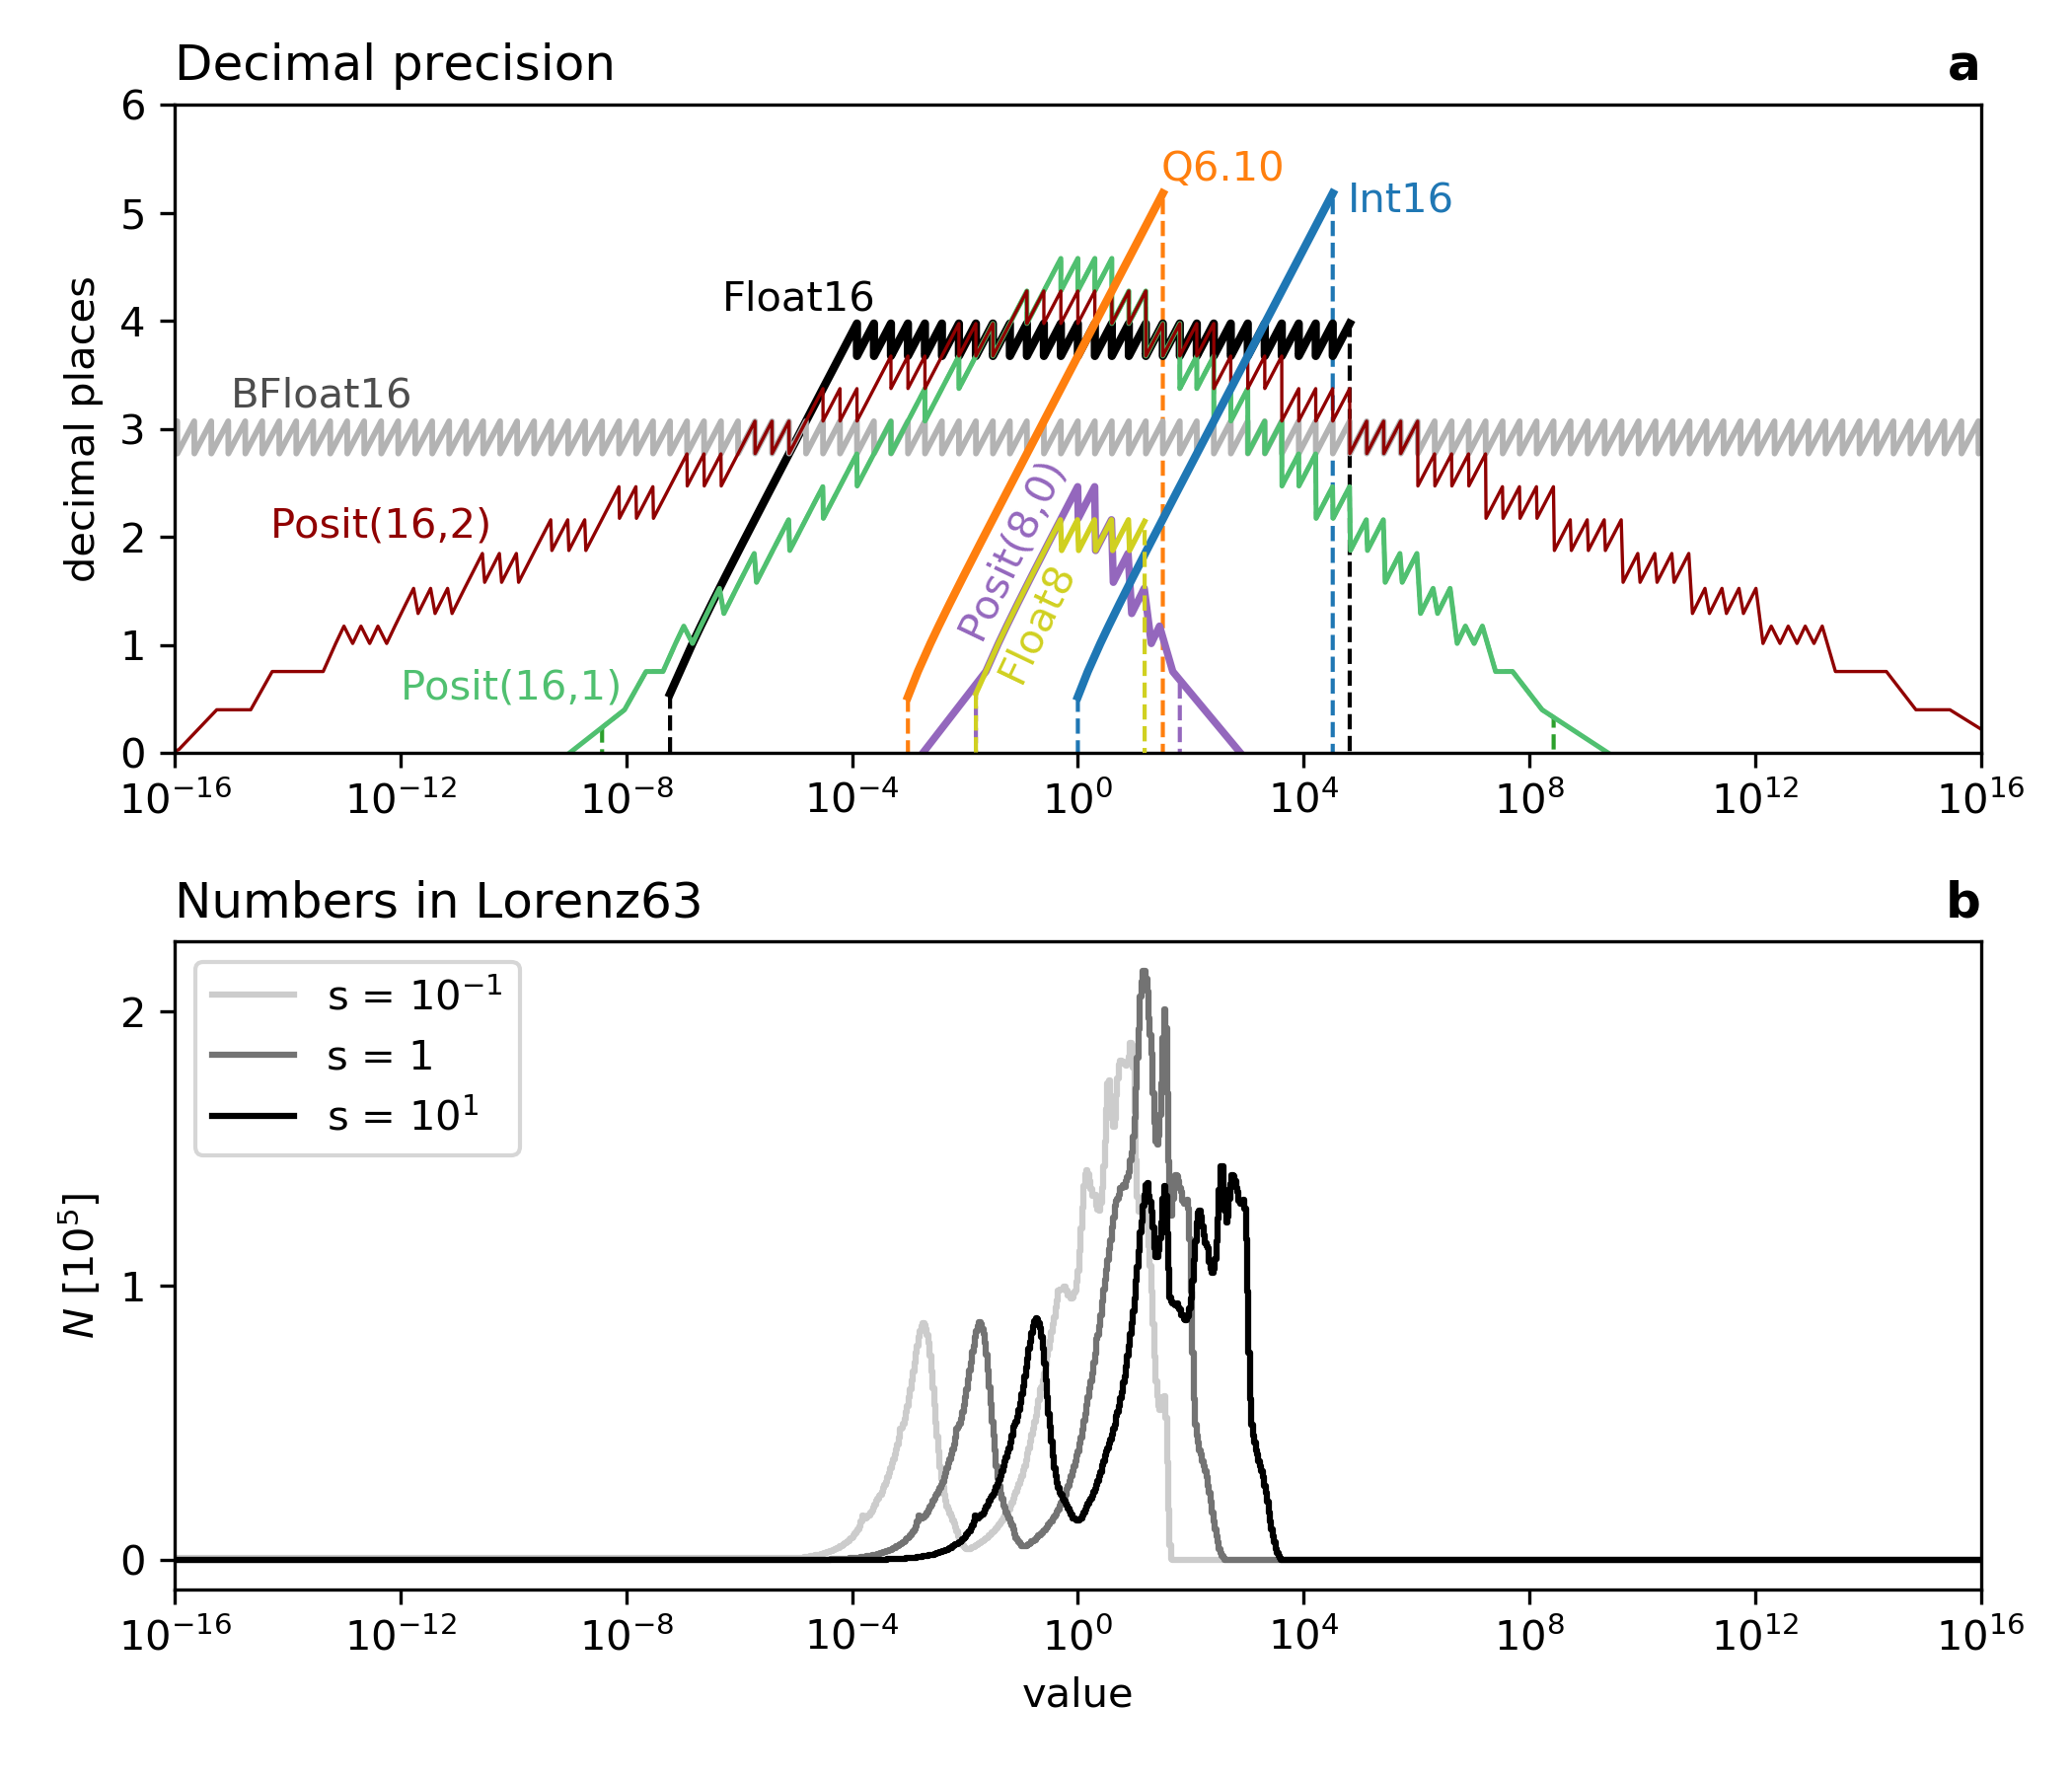
\includegraphics[width=1\textwidth]{../plots/decimal_precision.png}
\caption{(a) Decimal precision of various number formats. Dashed vertical lines indicate the range of representable numbers for each format. Float64, Float32 and Posit32 are beyond the axes limits. (b) Histogram of results of all arithmetic operations in the rescaled Lorenz system, considering absolute values.}
\label{fig:dec_acc}
\end{figure}

Fig. \ref{fig:dec_acc}a compares the worst-case decimal precision for various 16 and 8bit floats and posits, as well as 16bit integers and the fixed-point format Q6.10 (6 integer bits, 10 fraction bits). Float16 has a nearly constant decimal precision of almost 4 decimal places, which decreases for the subnormal numbers towards the smallest representable number $minpos$. 16bit posits, on the other hand, show an increased decimal precision for numbers around 1 and a wider dynamic range, in exchange for less precision for numbers on the order of $10^4$ as well as $10^{-4}$.  The machine error $\epsilon$, defined as half the distance between 1 and the next representable number, can be given in terms of decimal precision and is summarized in Table \ref{tab:formats} for the various formats. Due to the no overflow/no underflow-rounding mode, the decimal precision is slightly above zero outside the dynamic range. 

The decimal precision of 16bit integers is negative infinity for any number below 0.5 (round to 0) and maximised for the largest representable integer $2^{15} - 1 =  32767$. Similar conclusions hold for the fixed-point format Q6.10, as the decimal precision is shifted towards smaller numbers by a factor of $\tfrac{1}{2}$ for each additional fraction bit. This indicates problems for reduced precision modelling: Rescaling of the equations is desired to place many arithmetic calculations near the largest representable number, however, any result beyond will lead to disastrous results, as integer overflow usually returns a negative value following a wrap around behaviour. Flexibility regarding the dynamic range can be achieved with integer arithmetic if fixed point numbers are used \cite{Russell2017}. However, we did not achieve convincing results with integer arithmetic for the applications in this study.

\begin{table}
\center
\begin{tabular}{l | r | r | l | l | r | r}
Format & bits & exp bits & minpos & maxpos & $\epsilon$ &  \% NaR \\
\hline
Float64	& 64 & 11 & $5.0 \cdot 10^{-324}$ & $1.8 \cdot 10^{308}$  & 16.3 & 0.0 \\
Float32	& 32 & 8 & $1.0 \cdot 10^{-45}$ & $3.4 \cdot 10^{38}$ & 7.6 & 0.4 \\
Float16	& 16 & 5 & $6.0 \cdot 10^{-8}$ & 65504 & 3.7 & 3.1 \\
BFloat16	& 16 & 8 & $ 1.0 \cdot 10^{-45}$ & $3.4 \cdot 10^{38}$ & 2.8 & 0.4  \\
Posit32	& 32 & 2 &  $7.5 \cdot 10^{-37}$ & $7.5 \cdot 10^{37}$ & 8.8 & 0.0 \\
Posit(16,1) & 16 & 1 & $3.7 \cdot 10^{-9}$ & $3.7 \cdot 10^{9}$ & 4.3 & 0.0\\
Posit(16,2) & 16 & 2 & $1.4 \cdot 10^{-17}$ & $1.4 \cdot 10^{17}$ & 4.0 & 0.0\\
Posit(8,0) & 8 & 0 & $1.5 \cdot 10^{-2}$ & 64 & 2.2 & 0.4  \\
Float8 & 8 & 3 & $1.5 \cdot 10^{-2}$ & 15.5 & 1.9 &12.5\\
\end{tabular}
\vspace{10pt}
\caption{Some characteristics of various number formats. minpos is the smallest representable positive number, maxpos the largest. The machine error $\epsilon$ is here given as decimal precision. \% NaR denotes the percentage of bit patterns that represent not a number (NaN), infinity or not a real (NaR).}
\label{tab:formats}
\end{table}


\section{Lorenz 1963 system}
\label{sec:L63}

\subsection{Methods}
\label{sec:L63_methods}

The Lorenz system (L63, \cite{Lorenz1963}) is a chaotic attractor and serves as a simplistic model for atmospheric convection. It is an extensively studied toy model for forecast uncertainty \cite{Lorenz1963,Kwasniok2014,Jeffress2017,Tantet2018} and is used here to investigate the accumulation of rounding errors in the numerical integration of a chaotic system. The Lorenz system consists of the variables $x$,$y$ and $z$ that are described by the following non-linear differential equations
\begin{subequations}
\begin{align}
\frac{dx}{dt} &= \sigma(y-x) \\
\frac{dy}{dt} &= x(\rho - z) - y \\
\frac{dz}{dt} &= xy - \beta z
\end{align}
\label{eq:L63}%
\end{subequations}
with the typical parameter choices $\sigma = 10, \rho = 28$ and $\beta = \tfrac{8}{3}$, that permit chaotic behaviour. 

To find the optimal number representation to solve Eq. \ref{eq:L63} requires considering the dynamic range of all intermediate calculations. It is possible to influence this dynamic range using a \emph{rescaling} of the equations via a simple multiplication of the variables with a constant rescaling factor $s$. The rescaled variables are denoted as $\tilde{x} = sx$, and similarly for $\tilde{y},\tilde{z}$. Fig. \ref{fig:dec_acc}b shows histograms for all numbers that are used to solve the Lorenz system (including intermediate calculations). A comparison to the decimal precision in Fig. \ref{fig:dec_acc}a reveals the benefit of rescaling, especially for posit arithmetic: To profit from the increased decimal precision around 1, a scaling with $1/10$ is proposed to shift most calculations towards the centre of the dynamic range of representable numbers. Due to the constant decimal precision for floats, rescaling is less relevant for float arithmetic as long as no overflow nor underflow occurs. For integers, on the other hand, the Lorenz equations should be upscaled by a factor of approximately $100$, to shift the range of numbers to a higher decimal precision.

We solve the equations using a fourth order Runge-Kutta method \cite{Butcher2008}. Each substep in the time integration can be written as 
\begin{subequations}
\begin{align}
\tilde{x}^{n+1} &= \tilde{x}^n + RK_x\left(\tilde{y}^n-\tilde{x}^n\right) \\
\tilde{y}^{n+1} &= \tilde{y}^n + RK_y\left(\tilde{x}^n(\rho - \frac{\tilde{z}^n}{s}) - \tilde{y}^n \right) \\
\tilde{z}^{n+1} &= \tilde{z}^n + RK_z\left(\tilde{x}^n\frac{\tilde{y}^n}{s} - \beta \tilde{z}^n\right)
\end{align}
\label{eq:L63s}%
\end{subequations}
where $RK_x,RK_y,RK_z$ contain the Runge-Kutta coefficient and the time step $\Delta t$.  $RK_x$ also contains the parameter $\sigma$. The superscripts $n$ and $n+1$ denote the current and next substep.

The rescaling of the Lorenz system has its limitations: The non-linear terms in Eq. \ref{eq:L63s} involve a division by the scaling constant $s$, which leads to the result of the arithmetic operations $\tfrac{\tilde{z}}{s}, \rho - \tfrac{\tilde{z}}{s},$ and $\tfrac{\tilde{y}}{s}$ being invariant under scaling. This is observed in the histograms of arithmetic results (Fig. \ref{fig:dec_acc}b), as high counts of values between 1 and 50 exist for different choices of $s$. A changing shape of the histogram with $s$ is a consequence. Following these results an underlying challenge of reduced precision modelling becomes apparent: One has either to find a number format that fits the range of computed numbers, or rescale the equations to optimise their range for a given number format.

\subsection{Results}
\label{sec:lorenz}


\begin{figure}
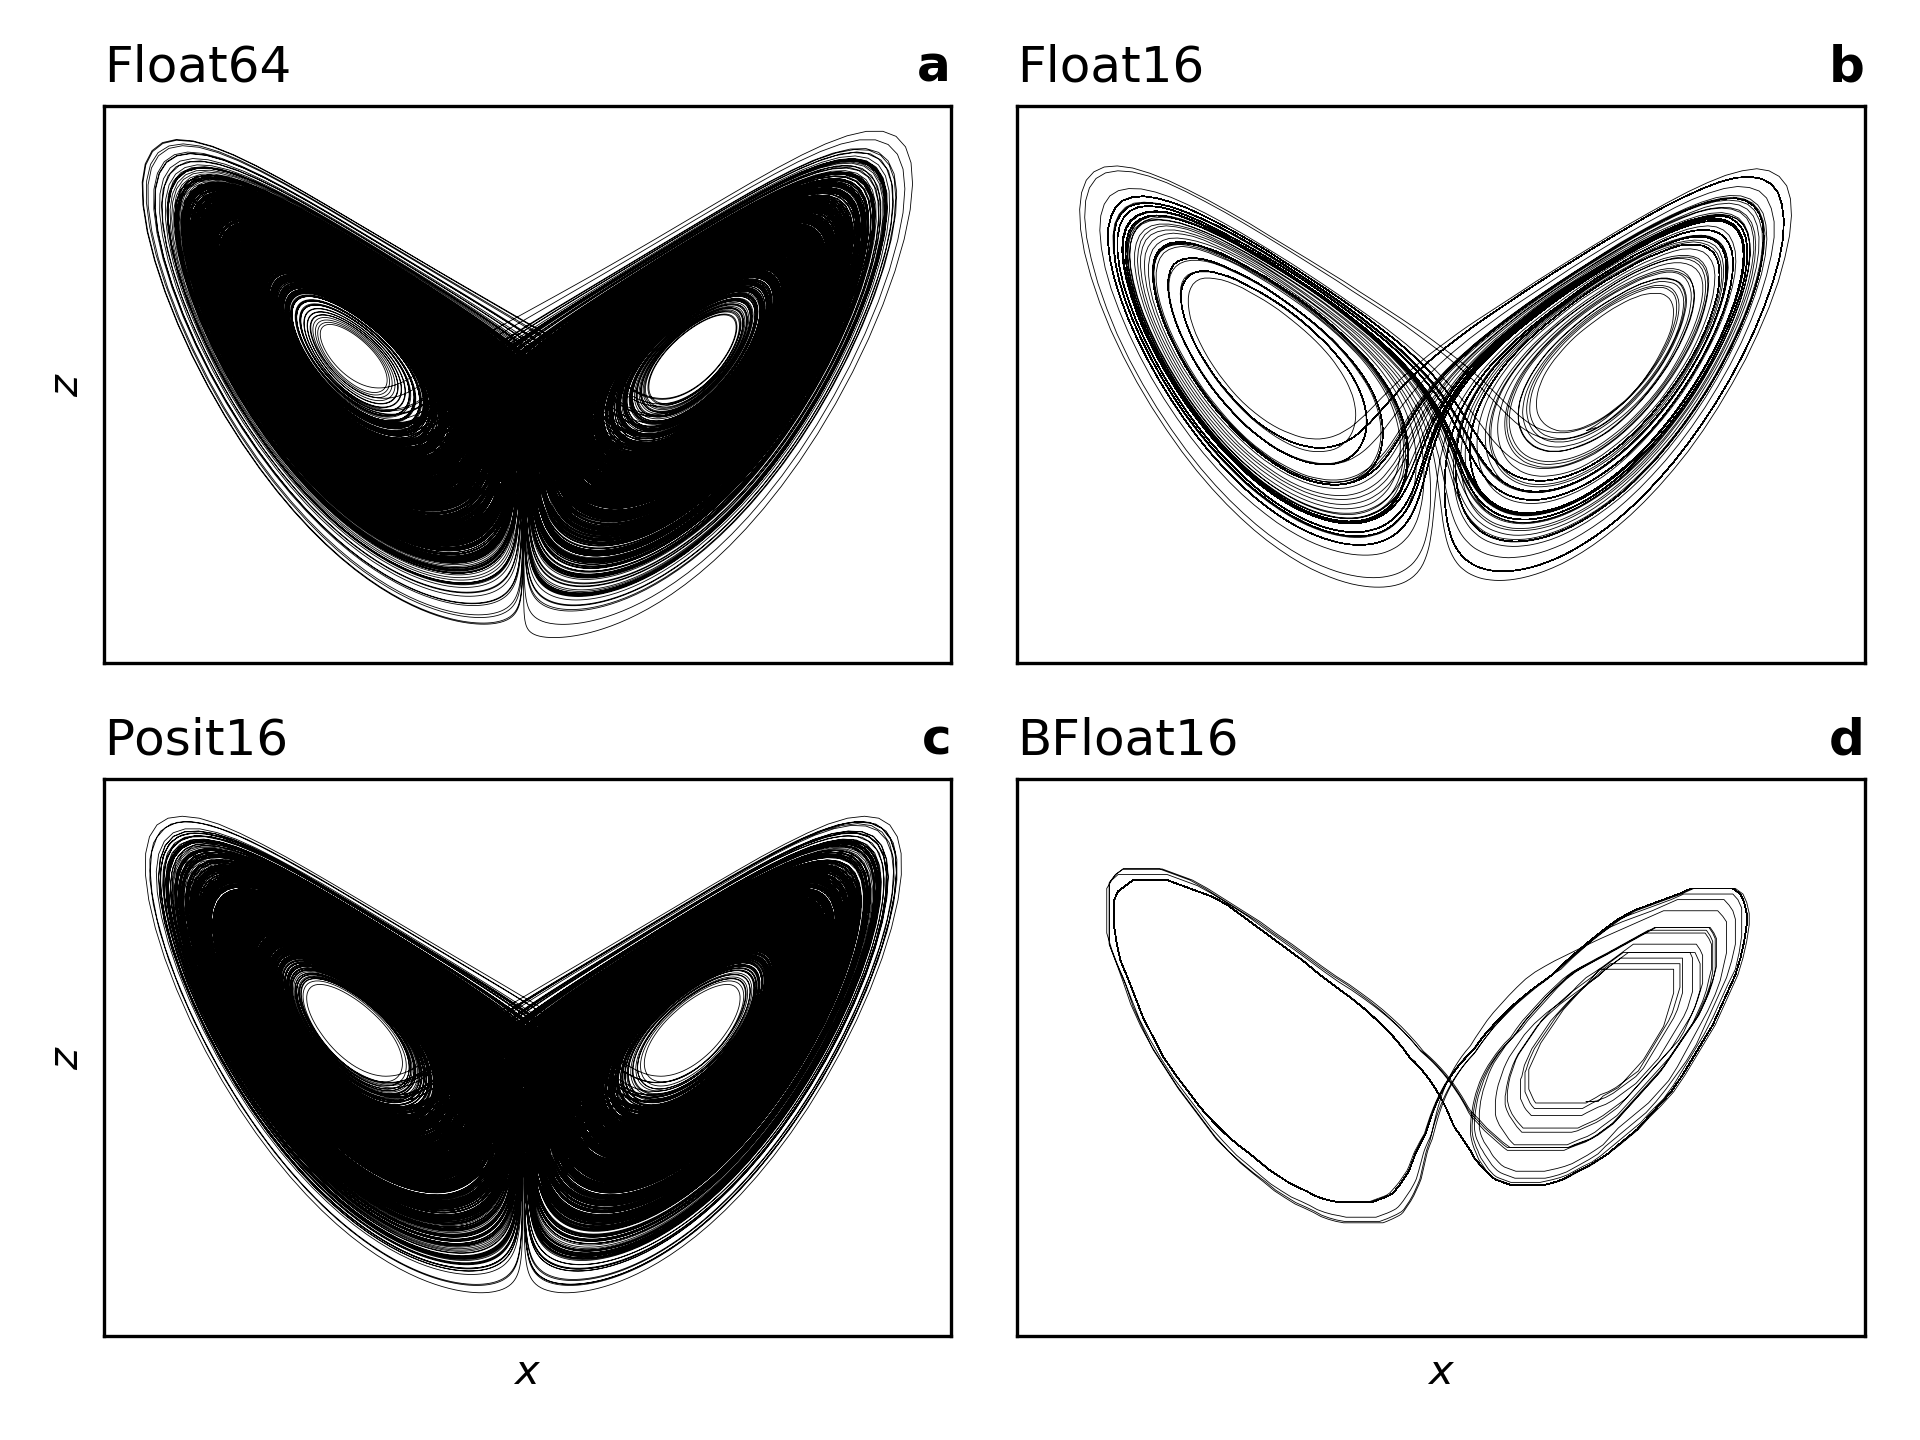
\includegraphics[width=1\textwidth]{../plots/lorenz_attractor.png}
\caption{The Lorenz attractor computed with different number formats. The scaling of the Lorenz equations (Eq. \ref{eq:L63s}) is (a,b,d) $s=1$, (c) $s=0.1$. All trajectories are integrated from the same initial conditions for 100,000 time-steps with spacing $\Delta t = 0.08$.}
\label{fig:L63}
\end{figure}

Regardless of the initial conditions, the Lorenz system will evolve towards a set of $(x,y,z)$ points called attractor (the x,z-section of the attractor is shown in Fig. \ref{fig:L63}a). This attractor is \emph{strange}, i.e. its geometric structure cannot be described in two dimensions, but is of fractal nature. 
While points on the model trajectory will get infinitesimally close to each other, the trajectory of the analytical Lorenz system will never repeat itself. However, if the model is discretised and if the variables are represented with finite precision, only a finite amount of distinct states can be represented and the model trajectory will necessarily repeat itself if integrated for long enough. 

Integrating the Lorenz system with half precision floats yields an attractor that is repeating itself fairly early and the space that is filled by the line of the trajectory is significantly smaller when compared to the space of a trajectory with double precision (compare Fig. \ref{fig:L63}a and b). However, when using posits and a rescaling factor of $s=0.1$ the representation of the attractor is improved significantly (Fig. \ref{fig:L63}c). The results for posits looks similar to the results with 16-bit floats if no rescaling was used (not shown here). The solution of the Lorenz system with integers fails to represent the true dynamics as the model converges to the origin (Fig. \ref{fig:L63}d).

We have calculated the so-called \emph{fractal dimension} as a diagnostic to quantify the fidelity of simulations of the discretised Lorenz equations when different number formats are used. The fractal dimension quantifies how space-filling an attractor is. Using a box-counting algorithm, we estimate the dimension of the posit attractor to be 1.78, whereas the half precision float attractor is only 1.29, compared to the true value of approximately 2.06 \cite{Grassberger1983,McGuinness1983}. 


\section{Shallow water model}
\label{sec:swm}

\subsection{Methods}
\label{sec:swm_methods}

This section will evaluate the different number formats (16-bit half precision floats, 16-bit posits with 0,1 or 2 exponent bits) when solving the shallow water equations. The shallow water equations result from a vertical integration of the Navier-Stokes equations under the assumption that horizontal length scales are much greater than vertical scales. This assumption holds for many features of the general circulation of atmosphere and ocean \cite{Gill1982,Vallis2006}. The shallow water equations for the prognostic variables velocity $\mathbf{u} = (u,v)$ and sea surface elevation $\eta$ are
\begin{subequations}
\begin{align}
\frac{\partial \mathbf{u}}{\partial t} &+ (\mathbf{u} \cdot \nabla) \mathbf{u} + f\hat{\mathbf{z}} \times \mathbf{u} = -g\nabla \eta + \mathbf{D} + \mathbf{F} \\
\frac{\partial \eta}{\partial t} &+ \nabla \cdot (\mathbf{u}h) = 0.
\end{align}
\label{eq:swe}%
\end{subequations}
For the atmosphere, $\eta$ is interpreted as pressure \cite{Gill1982}. The shallow water system is forced with a zonal wind stress $\mathbf{F}$. The dissipation term $\mathbf{D}$ removes energy on large scales (bottom friction) and on small scales (diffusion). The non-linear term $(\mathbf{u} \cdot \nabla) \mathbf{u}$ represents advection of momentum. The term $f\hat{\mathbf{z}} \times \mathbf{u}$ is the Coriolis force and $-g\nabla \eta$ is the pressure gradient force, with $g$ being the gravitational acceleration. Eq. \ref{eq:swe}b is the shallow water-variant of the continuity equation, ensuring conservation of mass. The domain is a zonally periodic rectangular channel of size $2000\op{km} \times 1000\op{km}$, with a meridional mountain ridge in the middle of the domain. A more detailed description of the shallow water model, introducing the remaining parameters and variables in Eq. \ref{eq:swe}, is presented in appendix \ref{sec:app}. The shallow water equations are discretised using 2nd order centred finite differences on an Arakawa C-grid \cite{Arakawa1977} with a grid spacing of $\Delta = 20\operatorname{km}$ (100x50 grid points) and the Runge-Kutta fourth order method \cite{Butcher2008} is used for time integration. The advection terms are discretised using an energy and enstrophy conserving scheme \cite{Arakawa1990}. 

To also test the use of the different number formats for the representation of passive tracers in atmosphere and ocean, we extend the shallow water equations with an advection equation. Tracers could, for example, be temperature and salinity in the ocean or aerosols in the atmosphere, which are regarded here, for simplicity, as passive (i.e. they do not influence the flow). The change of the distribution of a passive tracer $q$ that is advected by the underlying flow field is described by
\begin{equation}
\frac{\partial q}{\partial t} + \mathbf{u} \cdot \nabla q = 0.
\label{eq:adv}
\end{equation}
We discretise Eq. \ref{eq:adv} with a semi-Lagrangian advection scheme \cite{Smolarkiewicz1992}, which calculates the tracer concentration for a given grid cell from the concentration at the previous time step at a departure point, which is determined from the flow field. As the departure point is in general in between grid nodes an interpolation is required to find the concentration at the departure point. The discretisation of Eq. \ref{eq:adv} is therefore turned into an interpolation problem.

For reduced precision it is essential to rescale the shallow water equations to avoid arithmetic operations with very large or very small results, as the dynamic range of representable numbers is limited (Fig. \ref{fig:dec_acc}a). This is especially true for some sophisticated schemes like the biharmonic diffusion \cite{Griffies2000}, which is often used to remove energy from the grid scale to ensure numerical stability. For biharmonic diffusion a fourth derivative in space is calculated. Due to the large dimension of geophysical applications, this term can get very small $\mathcal{O}(10^{-20})$ while viscosity coefficients are typically very large $\mathcal{O}(10^{11})$. The prognostic variables of Eq. \ref{eq:swe} and \ref{eq:adv} are typically $\mathcal{O}(1\op{ms}^{-1})$ for $\mathbf{u}$, $\mathcal{O}(1\op{m})$ for $\eta$ and $\mathcal{O}(1)$ for $q$. We can therefore retain their physical units in the discretised numerical model. However, due to the grid spacing $\Delta$ being large for geophysical flows, we need to use dimensionless Nabla operators $\tilde{\nabla} = \Delta\nabla$. The continuity equation Eq. \ref{eq:swe}b, for example, is discretised with an explicit time integration method as
\begin{equation}
\eta^{n+1} = \eta^n + RK_{\eta}\left( - \tilde{\nabla} \cdot (\mathbf{u}h)^n\right)
\end{equation}
where $RK_\eta$ is the Runge-Kutta coefficient times $\tfrac{\Delta t}{\Delta}$ which is precomputed at high precision, to avoid a division by a large value $\Delta$ and a subsequent multiplication with a large value for $\Delta t$. The other terms are rescaled accordingly ($\tilde{f} = f\Delta$; $\tilde{\mathbf{F}} = \mathbf{F}\Delta$; please see appendix \ref{sec:app} for a discussion of the dissipation term $\mathbf{D}$). The entire numerical integration is performed using the various reduced precision number formats. However, posits are converted back to single precision floats for model output and some of the forcing and boundary terms that remain constant throughout the model integration are computed at higher precision during model initialisation to avoid problems with the dynamic range.


\subsection{Results}

\begin{figure}
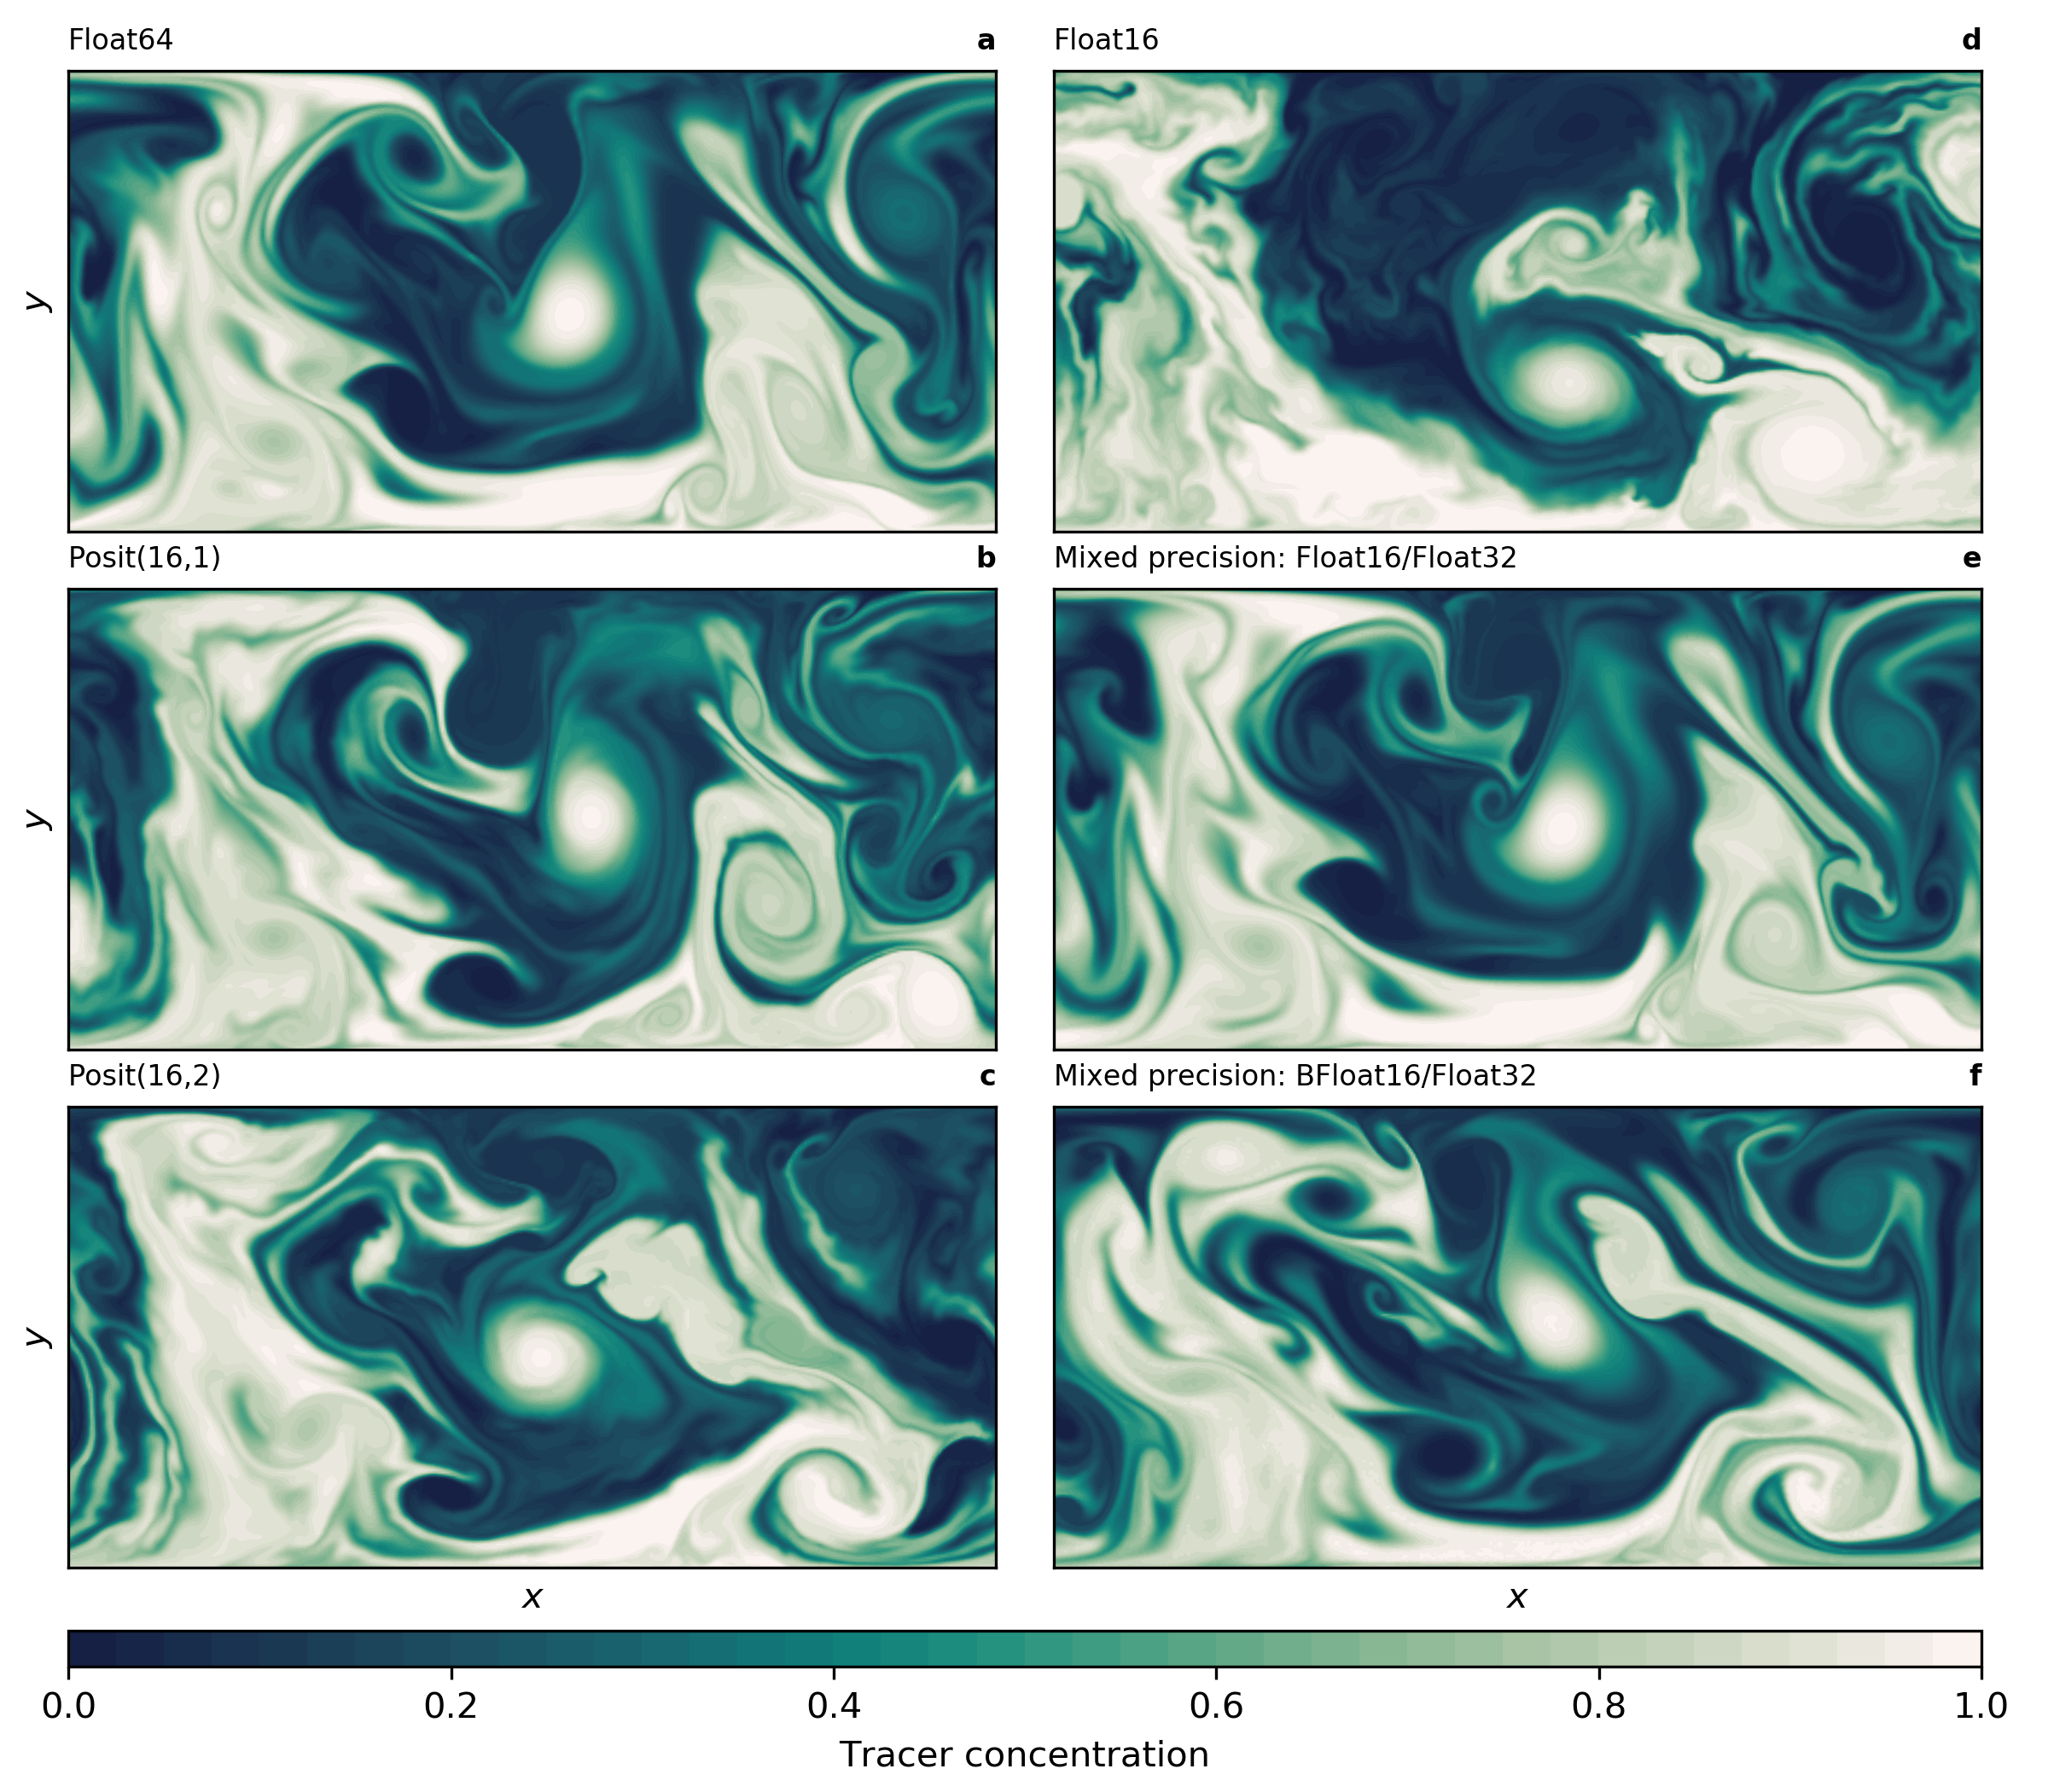
\includegraphics[width=1\textwidth]{../plots/snapshot.png}
\caption{Snapshot of tracer concentration simulated by the shallow water model using different 16bit number formats. Mixed precision using Float32 for the prognostic variables only is used for (e) and (f). The tracer was injected uniformly in the lower half of the domain 50 days before. This simulation was run at a resolution of $\Delta = 5$km (400x200 grid points).}
\label{fig:snapshot}
\end{figure}

The solution to the shallow water equations includes vigorous turbulence that dominates a meandering zonal current. Using either float or posit arithmetic with 16 bit the simulated fluid dynamics are very similar to a double precision reference: As shown in a snapshot of tracer concentration (Fig. \ref{fig:snapshot}) stirring and mixing can be well simulated with half precision floats and with 16-bit posits (2 exponent bits). However, the half precision simulation (Fig. \ref{fig:snapshot}c) deviates much faster than the posit simulation (Fig. \ref{fig:snapshot}b) from the double precision reference (Fig. \ref{fig:snapshot}a). This provides a first evidence that the accumulated rounding errors with posits are smaller than with floats. Only the posit simulations without exponent bit suffer from numerical instabilities, due to the limited dynamic range (Fig. \ref{fig:dec_acc}a). 

\begin{figure}
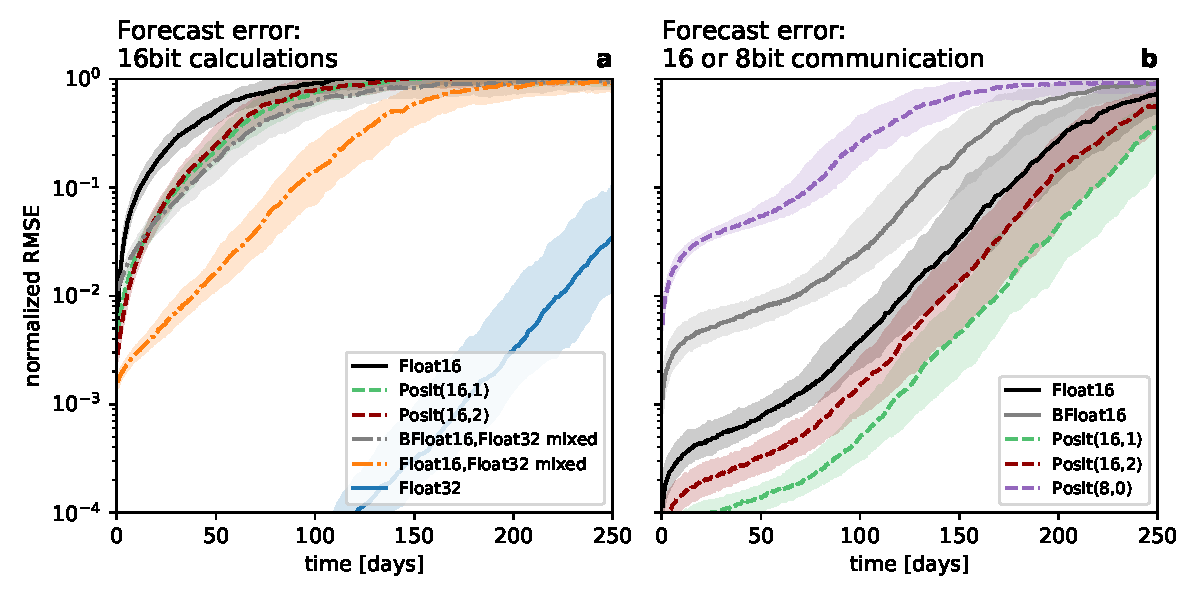
\includegraphics[width=1\textwidth]{../plots/rmse_eta.pdf}
\caption{Forecast error measured as the root mean square error (RMSE) of sea surface height $\eta$ taking Float64 as reference. (a) Forecast error for various 16bit number formats and mixed 16bit/32bit simulations for which the prognostic variables are kept at Float32. (b) Forecast error for reduced precision communication in 8 or 16bit with various number formats used for encoding, with Float64 used for all calculations.  The communication of boundary values occurs at every time step for the prognostic variables. The RMSE is normalised by a mean forecast error at very long lead times. Solid lines represent the median of 200 forecasts per number format. The shaded areas denote the interquartile range of the ensemble.}
\label{fig:rmse}
\end{figure}

To quantify differences between reduced precision arithmetics we perform model forecasts that compare rounding errors. The forecast error in the shallow water model is computed as root mean square error (RMSE) taking the model based on double precision floating-point arithmetics as reference truth. We use the sea surface height (equivalent to pressure) to compute the forecast error as this variable captures the large scale circulation. The forecasts are created based on 280 different initial conditions from random start dates of a 50 year long control simulation. Each forecast is performed several times from identical initial conditions but with the various number formats. To compare the magnitude of rounding error that are caused by a reduction in precision to a realistic level of error that is caused by model discretisation, we also perform forecasts at double precision that fall back to a 3rd-order Runge-Kutta scheme for time integration and a simpler enstrophy conserving advection scheme described in \citeA{Sadourny1975}. Both advection schemes have the same continuous formulation, but the \citeA{Arakawa1990} advection scheme has a wider stencil. We normalise the RMSE by the climatological mean forecast error at very long lead times. A normalised RMSE of 1 therefore means that all information of the initial conditions is removed by chaos.

Clearly the best forecast is obtained for posit arithmetic with 1 or 2 exponent bits (Fig. \ref{fig:rmse}), with a small accumulation of rounding errors even for lead times of 100 days. The forecast error for 16-bit posits without exponent bit increases quickly (Fig. \ref{fig:rmse}), especially for short forecast lead times, but a persistence forecast, i.e. assuming the initial conditions persist over time, is still worse (not shown). Half precision floats outperform 16-bit posits without exponent bit, presumably due to the limited dynamic range of only 8 orders of magnitude compared to 12 for half precision floats (Fig. \ref{fig:dec_acc}a). The forecast error of half precision floats is larger than the discretisation error.

\begin{figure}
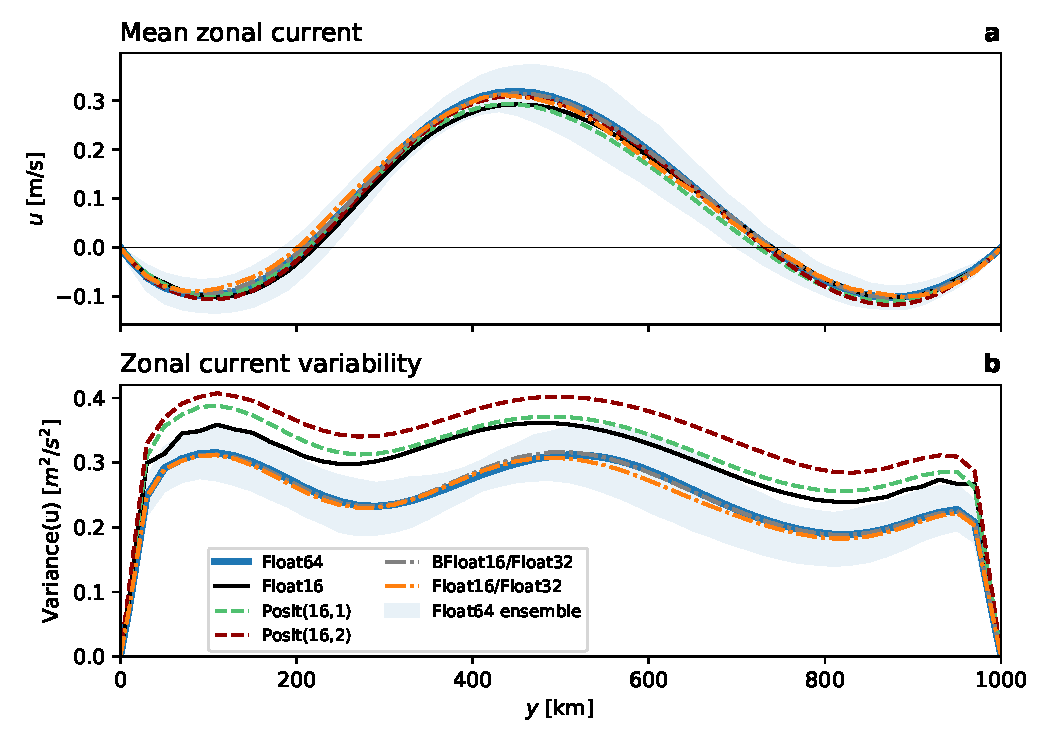
\includegraphics[width=1\textwidth]{../plots/meanvar_u.pdf}
\caption{Climatology and variability of the zonal current. (a) Zonally-averaged zonal current $u$ as a function of the meridional coordinate $y$. (b) Zonal variance of the zonal current as a function of $y$. Shaded areas denote the interquartile temporal variability around the (a) mean and (b) variance of reference simulation with Float64.}
\label{fig:mean}
\end{figure}

\begin{figure}
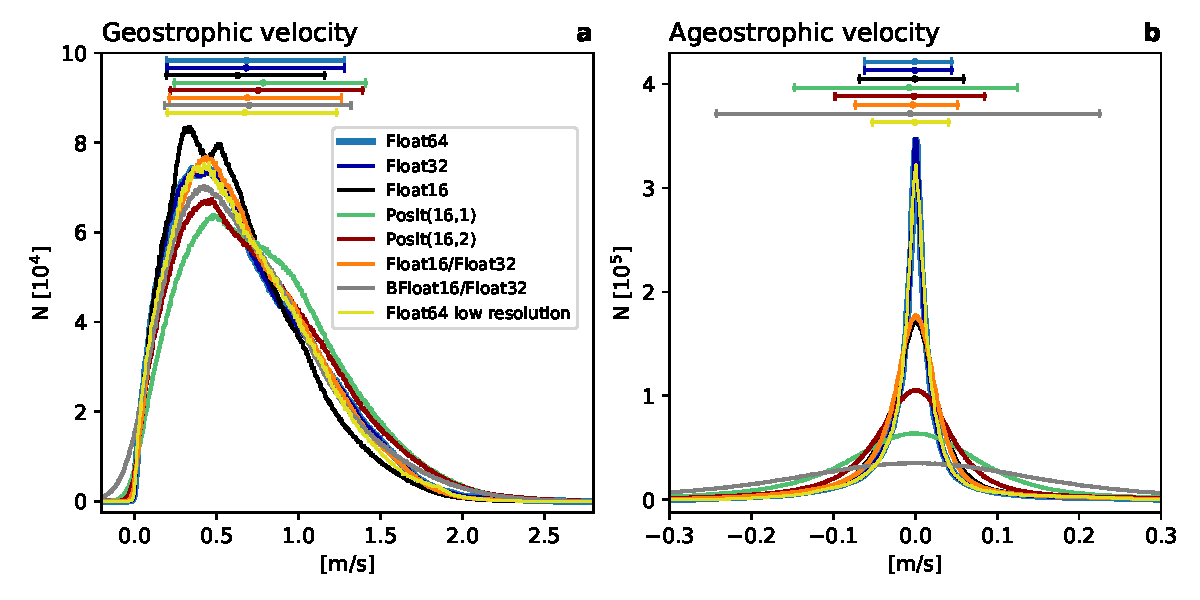
\includegraphics[width=1\textwidth]{../plots/ageostrophic.pdf}
\caption{Geostrophic balance as simulated with different number formats. (a) Histograms of flow-parallel components of geostrophic velocity. (b) as (a) but for the ageostrophic velocities. Horizontal bars denote the mean, 10th and 90th-percentile in respective colours.}
\label{fig:mean}
\end{figure}

%\begin{figure}
%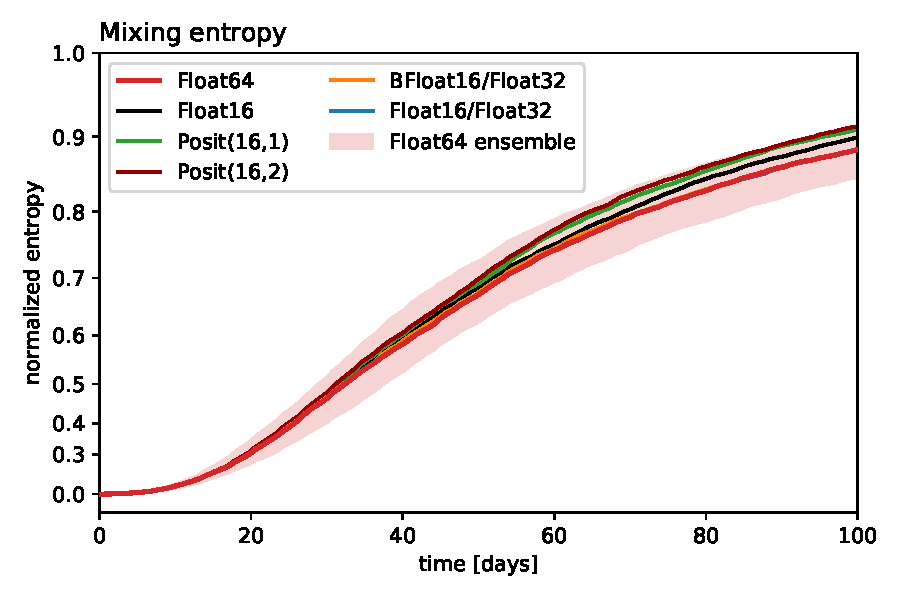
\includegraphics[width=1\textwidth]{../plots/entropy.pdf}
%\caption{Entropy of mixing calculated from the tracer concentration simulated with various 16bit number formats. The entropy is normalized by the entropy of a homogeneous tracer. Lines represent the mean of 200 forecasts per number format. The shaded area denotes the interquartile range of the reference ensemble simulations with Float64. Note the cubically scaled y-axis.}
%\label{fig:entropy}
%\end{figure}

\begin{figure}
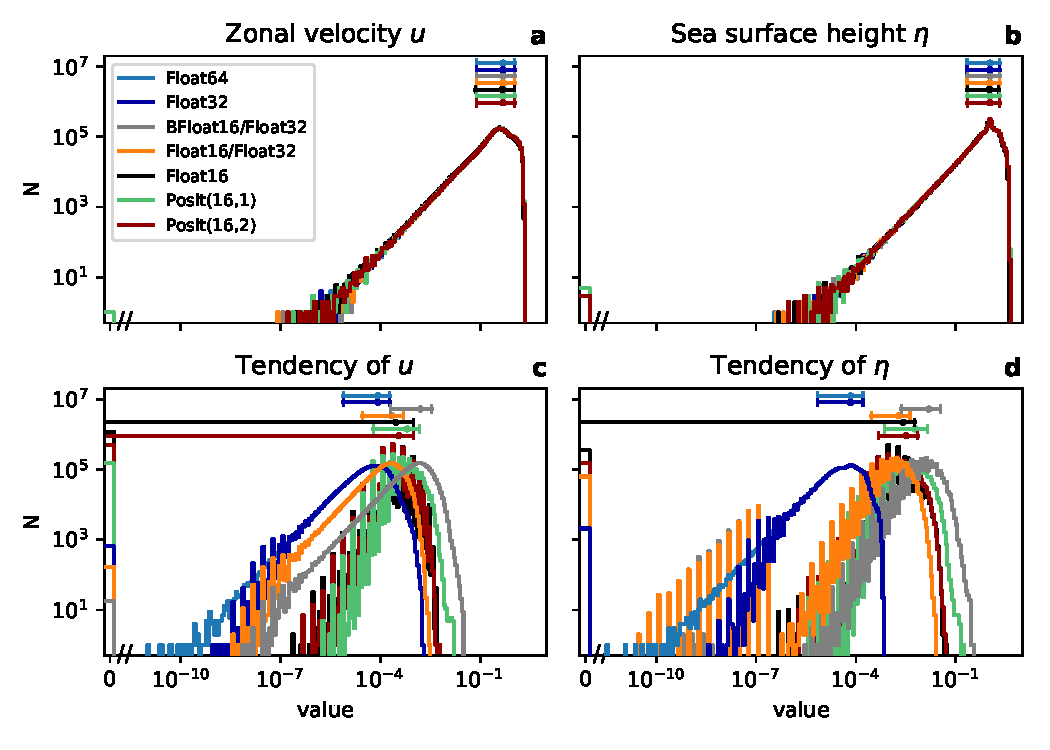
\includegraphics[width=1\textwidth]{../plots/tendency_hist.pdf}
\caption{Histograms of the numeric values of the prognostic variables (a) zonal velocity $u$, (b) meridional velocity $v$, (c) sea surface height $\eta$, and the respective tendencies of (d) $u$, (e) $v$, and (f) $\eta$, simulated with different 16, 32 and 64bit number formats. Mean, 10th and 90th percentile are shown above the histograms in respective colors. Note the break on the x-axis.}
\label{fig:tend}
\end{figure}

\subsection{Mixed precision arithmetic}
\label{sec:mixed}


\subsection{Reduced precision communication}
\label{sec:comm}

\begin{figure}
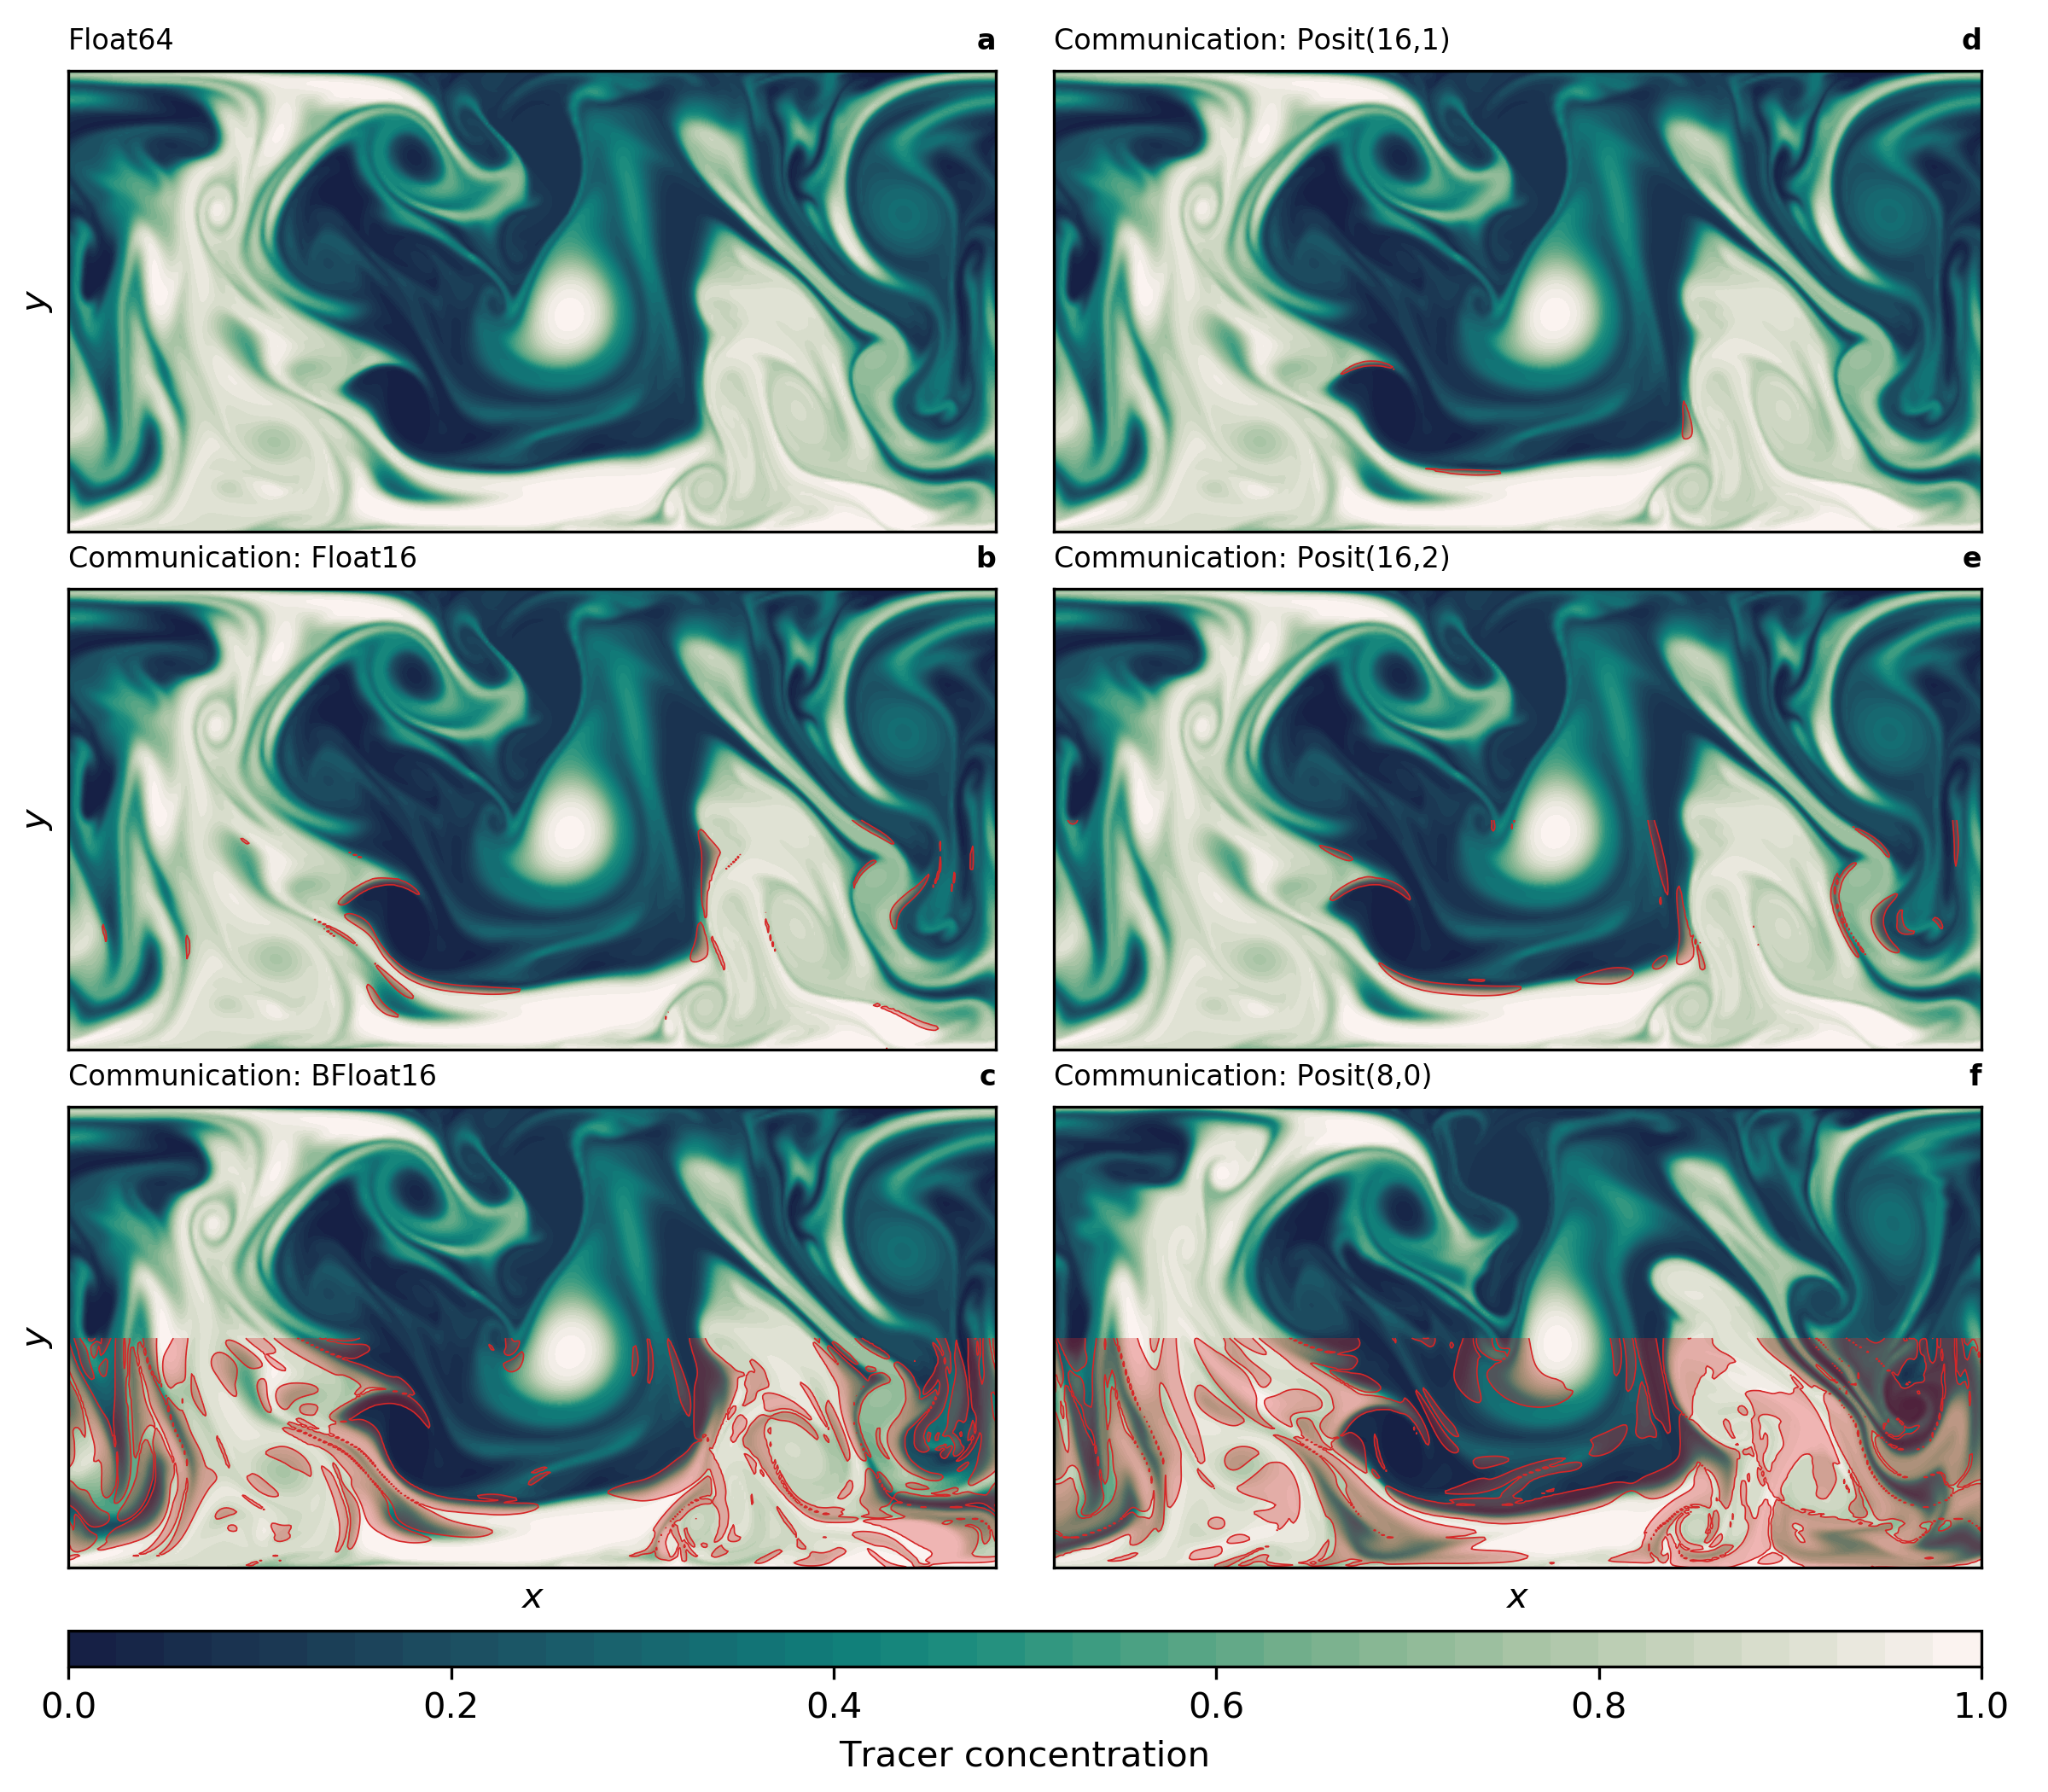
\includegraphics[width=1\textwidth]{../plots/snapshot_comm.png}
\caption{Snapshot of tracer concentration simulated by the shallow water model using reduced precision communication. The communication of boundary values occurs at every time step for the prognostic variables. Float64 was used for all calculations. Areas where the absolute error exceeds 0.05 are shaded in red only in the lower half of the domain. The tracer was injected uniformly in the lower half of the domain 50 days before. This simulation was run at a resolution of $\Delta = 5$km (400x200 grid points).}
\label{fig:snapshot_comm}
\end{figure}



\section{Discussion and Conclusion}
\label{sec:discuss}

Using a software emulator we have tested posit arithmetic for weather and climate simulations. The attractor of the Lorenz 1963 model, a chaotic but simplistic model of atmospheric convection, is considerably improved using 16-bit posits with one exponent bit when compared to 16-bit half precision floats. Half precision floats can be used to perform forecasts with the shallow water model, a two-dimensional fluid circulation model that represents either atmospheric or oceanic flows. However, 16-bit posits with either 1 or 2 exponents clearly outperform floats and appear very promising for application in high performance computing for Earth System modelling. Especially 16-bit posits with 2 exponent bits, that have a wide dynamic range of 32 orders of magnitude, are likely to be widely applicable. Running computationally very demanding algorithms at 16 bit could greatly reduce the wall-clock time for weather and climate simulations on future high performance computing architecture.

The numerical discretisation that was used in this paper, with a fully-explicit time stepping scheme and 2nd order centred finite differences, is common to solve the equations of motion in fluid dynamics. However, various different methods of discretisation exist, including spectral methods, finite element/volume and implicit time stepping. The requirements on reduced precision will differ for the different algorithms and some methods may be more sensitive to rounding errors compared to the techniques that were studied in this paper. However, there is no prior reason why floats should be superior to posits in these cases and the smaller rounding errors of 16-bit posits compared to half precision floats in our applications suggest that posits are very competitive. 
In contrast, the wider dynamic range of posits with 1 or 2 exponent bits compared to half precision floats will facilitate the application in more complex numerical models since it will become difficult to reduce the dynamic range of all intermediate operations for complex applications. While floating-point arithmetic is then prone to overflows or underflows, posit arithmetic will be able to tolerate very small and very large numbers, although decimal precision is decreasing away from 1 for posits.

We do not show results for the bfloat16 floating-point format in this paper as rounding errors destroy the dynamics of the shallow water model. Due to the 8 exponent bits the dynamic range of bfloat16 ($10^{-40}$ to $10^{38}$) remains the same as for single precision simulations. However, the small number of 7 fraction bits in this format causes rounding errors that inhibit the time evolution of the model.

In this paper, we perform model forecasts with a \emph{perfect model}. Any form of model error is ignored, as the double precision reference is exactly the same model as its reduced precision counterparts. Any form of initial condition error is also ignored. Only discretisation errors are estimated by changing the advection scheme to a simpler non-energy conserving form \cite{Sadourny1975} and by using a third-order instead of a fourth-order Runge-Kutta method. Here, we are likely underestimating the discretisation error of real models which also arises from the limited accuracy of spatial discretisation schemes. 

This is not a realistic set-up for weather or climate models. Real models include many other sources of forecast error (see section \ref{sec:intro}) and it is likely that the contributions of rounding errors from 16-bit arithmetic would be dwarfed by errors in initial conditions or discretisation errors in many applications. As the forecast error with 16-bit posits (1 or 2 exponent bits) are still considerably lower than the discretisation error, this suggest that simulations with posit arithmetic of even less than 16 bit may be feasible. However, as 8bit numbers are very likely unsuitable for applications in weather and climate models, we propose 16-bit posit with 2 exponent bits as a format that would likely meet the requirements of many algorithms used in weather and climate models. Together with a 32-bit posit format with 2 exponent bits (to match the dynamic range of single precision floats), a posit processor based on these two formats could greatly support the transition of models that are rewritten to use less than 32 bits to represent real numbers. We believe that high performance computing for Earth System modelling would benefit greatly from a processor that would support both 16 and 32-bit posit formats with 2 exponent bits.

\appendix
%%Appendix A
\section{Shallow water model}
\label{sec:app}

The shallow water equations are discretised on the $(x,y)$-plane over the rectangular domain $L_x \times L_y$. We associate $x$ with the zonal and $y$ with the meridional direction. The domain is centred at 45N and the beta-plane approximation \cite{Vallis2006} is used to linearize the Coriolis parameter which varies linearly from $7.27 \times 10^{-5}\op{s}^{-1}$ at the southern boundary to $9.25 \times 10^{-5}\op{s}^{-1}$ at the northern boundary. The boundary conditions are periodic in zonal direction and no-slip at the northern and southern boundary. The layer thickness is $h = \eta + H(x)$, with
\begin{equation}
H(x) = H_0 - H_1\exp\left(-H_\sigma^{-2}(x-\tfrac{L_x}{2})^2\right)
\end{equation}
being the undisturbed depth, representing a mountain ridge at $x=\tfrac{L_x}{2}$ spanning from the southern to the northern boundary. The standard depth is $H_0 = 500\op{m}$. The ridge has a height of $H_1 = 50\op{m}$. The characteristic width of the ridge is $H_\sigma = 300\op{km}$. The time step $\Delta t = 282\op{s}$ is chosen to resolve surface gravity waves, traveling at maximum phase speed $\sqrt{gH_0}$ with CFL number being 1 and gravitational acceleration $g=10\op{ms}^{-1}$. The wind stress forcing $\mathbf{F} = (F_x,0)$ is constant in time, acts only on the zonal momentum budget
\begin{equation}
Fx = \frac{F_0}{\rho h} \cos\left(\pi\left(y{L_y}^{-1} - 1\right)\right)^2
\end{equation}
and vanishes at the boundaries. The water density is $\rho = 1000\op{kg}\op{m}^{-3}$ and $F_0 = 0.12\op{Pa}$. The dissipation term $\mathbf{D}$ is the sum

\begin{equation}
\mathbf{D} = -r\mathbf{u} - \nu \nabla^4 \mathbf{u}
\end{equation}
of a linear bottom drag with time scale $r^{-1} = 300 \op{days} \approx 2.6 \times 10^7 \op{s}$ \cite{Arbic2008} and a biharmonic diffusion with viscosity coefficient $\nu \approx 1.33\times10^{11} \op{m}^4\op{s}^{-1}$ \cite{Griffies2000}. To avoid division and subsequent multiplication with large numbers throughout the numerical model integration, we use instead
\begin{equation}
\tilde{\mathbf{D}} = -\tilde{r}\mathbf{u} - \tilde{\nu}\tilde{\nabla}^4\mathbf{u}
\end{equation}
with $\tilde{r} = r\Delta \approx 0.0008\op{ms}^{-1}$,  and $\tilde{\nu} = \nu\Delta^{-3} \approx 0.16\op{ms}^{-1}$. Computing the term $\tilde{\mathbf{D}}$ instead of $\mathbf{D}$ is required to avoid arithmetic under and overflow with floats or huge rounding errors with posit arithmetic. 

The semi-Lagrangian advection scheme involves the computation of a departure point $\mathbf{x}_d$. In order to avoid large numbers of the coordinates ($L_x = 2 \cdot 10^6$m), we use instead a non-dimensional coordinate $\mathbf{\tilde{x}} = \mathbf{x}\Delta^{-1}$ to compute the departure point as 
\begin{equation}
\mathbf{\tilde{x}}_d = \mathbf{\tilde{x}}_a - \mathbf{u}_i \tfrac{\Delta t_\text{adv}}{\Delta}
\end{equation}
where $\mathbf{\tilde{x}}_a$ are the coordinates of the arrival grid node and $\mathbf{u}_i$ the velocity interpolated on the mid-point in space and time\cite{Smolarkiewicz1992}. The advective time step $\Delta t_\text{adv}$ is much larger than $\Delta t$ to reduce numerical diffusion of the tracer due to a smaller number of interpolations. In the simulations of Fig. \ref{fig:snapshot} ($\Delta = 10\op{km}$) the rescaled time step is $\tfrac{\Delta t_\text{adv}}{\Delta} \approx \tfrac{2 \cdot 10^4\op{s}}{10^4\op{m}} =  2 \op{sm}^{-1}$ and therefore precomputed.

%\section{Perspectives for quires}
%\label{sec:app2}
%Although we do not use quires throughout the simulations, for completeness we want to discuss computations that could greatly benefit from the use of quires. Summing the tendencies of the right-hand side of Eq. \ref{eq:swe}a involves computations like
%\begin{equation}
%u^{n+1} = u^{n} + RK_u \left( Qhv + \partial_xp + D_x + F_x \right)
%\end{equation}
%where $RK_u$ is a constant that includes the Runge-Kutta coefficient and the time step. $Qhv$ is the advection of potential vorticity, $\partial_xp$ is the gradient of the Bernoulli potential, $D_x$ is the $u$-component of bottom friction and diffusion and $F_x$ is the wind forcing. It is a priori not clear which of the terms $u^n, Qhv, \partial_xp, D_x$ or $F_x$ dominate the sum. Physically speaking, the shallow water model is often close to geostrophic balance, which means that the Coriolis term (which is included in $Qhv$) and the pressure gradient term (which is included in $\partial_xp$) oppose each other. In general, however, the dominating balance will vary in space and time and therefore it is only clear at runtime what the preferred order of addition is, which is crucial to reducing the rounding error. Using quires could solve this problem since quires will be able to reduce rounding errors greatly when performing intermediate operations. Quires may allow to perform the sum over different terms to calculate the right-hand side of the equations with a single rounding error due to 16-bit arithmetic when the final result for the new velocity value is stored.

%Similarly, on every time step the potential vorticity $Q = \tfrac{f + \partial_xv - \partial_yu}{h}$ is computed as
%\begin{equation}
%Q_{i,j} = \frac{f_{i,j} + v_{i+1,j} - v_{i-1,j} - u_{i,j+1}+ u_{i,j-1}}{h_{i,j}}.
%\label{eq:PV}
%\end{equation}
%In many cases we should expect the Coriolis term $f$ to be the leading order term and the differences of $u$ and $v$, respectively, are often small.   Again, only at runtime the preferred order is known and depends on space and time. Therefore, a single rounding error with quires could greatly improve the precision of this computation.

 



%%

%  Numbered lines in equations:
%  To add line numbers to lines in equations,
%  \begin{linenomath*}
%  \begin{equation}
%  \end{equation}
%  \end{linenomath*}



%% Enter Figures and Tables near as possible to where they are first mentioned:
%
% DO NOT USE \psfrag or \subfigure commands.
%
% Figure captions go below the figure.
% Table titles go above tables;  other caption information
%  should be placed in last line of the table, using
% \multicolumn2l{$^a$ This is a table note.}
%
%----------------
% EXAMPLE FIGURES
%
% \begin{figure}
% \includegraphics{example.png}
% \caption{caption}
% \end{figure}
%
% Giving latex a width will help it to scale the figure properly. A simple trick is to use \textwidth. Try this if large figures run off the side of the page.
% \begin{figure}
% \noindent\includegraphics[width=\textwidth]{anothersample.png}
%\caption{caption}
%\label{pngfiguresample}
%\end{figure}
%
%
% If you get an error about an unknown bounding box, try specifying the width and height of the figure with the natwidth and natheight options. This is common when trying to add a PDF figure without pdflatex.
% \begin{figure}
% \noindent\includegraphics[natwidth=800px,natheight=600px]{samplefigure.pdf}
%\caption{caption}
%\label{pdffiguresample}
%\end{figure}
%
%
% PDFLatex does not seem to be able to process EPS figures. You may want to try the epstopdf package.
%

%
% ---------------
% EXAMPLE TABLE
%
% \begin{table}
% \caption{Time of the Transition Between Phase 1 and Phase 2$^{a}$}
% \centering
% \begin{tabular}{l c}
% \hline
%  Run  & Time (min)  \\
% \hline
%   $l1$  & 260   \\
%   $l2$  & 300   \\
%   $l3$  & 340   \\
%   $h1$  & 270   \\
%   $h2$  & 250   \\
%   $h3$  & 380   \\
%   $r1$  & 370   \\
%   $r2$  & 390   \\
% \hline
% \multicolumn{2}{l}{$^{a}$Footnote text here.}
% \end{tabular}
% \end{table}

%% SIDEWAYS FIGURE and TABLE
% AGU prefers the use of {sidewaystable} over {landscapetable} as it causes fewer problems.
%
% \begin{sidewaysfigure}
% \includegraphics[width=20pc]{figsamp}
% \caption{caption here}
% \label{newfig}
% \end{sidewaysfigure}
%
%  \begin{sidewaystable}
%  \caption{Caption here}
% \label{tab:signif_gap_clos}
%  \begin{tabular}{ccc}
% one&two&three\\
% four&five&six
%  \end{tabular}
%  \end{sidewaystable}

%% If using numbered lines, please surround equations with \begin{linenomath*}...\end{linenomath*}
%\begin{linenomath*}
%\begin{equation}
%y|{f} \sim g(m, \sigma),
%\end{equation}
%\end{linenomath*}

%%% End of body of article

%%%%%%%%%%%%%%%%%%%%%%%%%%%%%%%%
%% Optional Appendix goes here
%
% The \appendix command resets counters and redefines section heads
%
% After typing \appendix
%
%\section{Here Is Appendix Title}
% will show
% A: Here Is Appendix Title
%
%\appendix
%\section{Here is a sample appendix}

%%%%%%%%%%%%%%%%%%%%%%%%%%%%%%%%%%%%%%%%%%%%%%%%%%%%%%%%%%%%%%%%
%
% Optional Glossary, Notation or Acronym section goes here:
%
%%%%%%%%%%%%%%
% Glossary is only allowed in Reviews of Geophysics
%  \begin{glossary}
%  \term{Term}
%   Term Definition here
%  \term{Term}
%   Term Definition here
%  \term{Term}
%   Term Definition here
%  \end{glossary}

%
%%%%%%%%%%%%%%
% Acronyms
%   \begin{acronyms}
%   \acro{Acronym}
%   Definition here
%   \acro{EMOS}
%   Ensemble model output statistics
%   \acro{ECMWF}
%   Centre for Medium-Range Weather Forecasts
%   \end{acronyms}

%
%%%%%%%%%%%%%%
% Notation
%   \begin{notation}
%   \notation{$a+b$} Notation Definition here
%   \notation{$e=mc^2$}
%   Equation in German-born physicist Albert Einstein's theory of special
%  relativity that showed that the increased relativistic mass ($m$) of a
%  body comes from the energy of motion of the body—that is, its kinetic
%  energy ($E$)—divided by the speed of light squared ($c^2$).
%   \end{notation}




%%%%%%%%%%%%%%%%%%%%%%%%%%%%%%%%%%%%%%%%%%%%%%%%%%%%%%%%%%%%%%%%
%
%  ACKNOWLEDGMENTS
%
% The acknowledgments must list:
%
% >>>>	A statement that indicates to the reader where the data
% 	supporting the conclusions can be obtained (for example, in the
% 	references, tables, supporting information, and other databases).
%
% 	All funding sources related to this work from all authors
%
% 	Any real or perceived financial conflicts of interests for any
%	author
%
% 	Other affiliations for any author that may be perceived as
% 	having a conflict of interest with respect to the results of this
% 	paper.
%
%
% It is also the appropriate place to thank colleagues and other contributors.
% AGU does not normally allow dedications.


\acknowledgments
 The authors would like to thank Cerlane Leong and Mos\`{e} Giordano who contributed to \emph{SoftPosit.jl}. Milan Kl\"{o}wer and Tim N. Palmer gratefully acknowledge funding by the European Research Council under grant number 741112 \emph{An Information Theoretic Approach to Improving the Reliability of Weather and Climate Simulations}. Milan Kl\"{o}wer is also funded by NERC grant number NE/L002612/1.  Peter D. D\"{u}ben gratefully acknowledges funding from the Royal Society for his University Research Fellowship as well as funding from the ESIWACE project. ESIWACE has received funding from the European Union's Horizon 2020 research and innovation program under grant agreement 675191.

%% ------------------------------------------------------------------------ %%
%% References and Citations

%%%%%%%%%%%%%%%%%%%%%%%%%%%%%%%%%%%%%%%%%%%%%%%
%
% \bibliography{<name of your .bib file>} don't specify the file extension
%
% don't specify bibliographystyle
%%%%%%%%%%%%%%%%%%%%%%%%%%%%%%%%%%%%%%%%%%%%%%%

\bibliography{bibliography.bib}



%Reference citation instructions and examples:
%
% Please use ONLY \cite and \citeA for reference citations.
% \cite for parenthetical references
% ...as shown in recent studies (Simpson et al., 2019)
% \citeA for in-text citations
% ...Simpson et al. (2019) have shown...
%
%
%...as shown by \citeA{jskilby}.
%...as shown by \citeA{lewin76}, \citeA{carson86}, \citeA{bartoldy02}, and \citeA{rinaldi03}.
%...has been shown \cite{jskilbye}.
%...has been shown \cite{lewin76,carson86,bartoldy02,rinaldi03}.
%... \cite <i.e.>[]{lewin76,carson86,bartoldy02,rinaldi03}.
%...has been shown by \cite <e.g.,>[and others]{lewin76}.
%
% apacite uses < > for prenotes and [ ] for postnotes
% DO NOT use other cite commands (e.g., \citet, \citep, \citeyear, \nocite, \citealp, etc.).
%



\end{document}



More Information and Advice:

%% ------------------------------------------------------------------------ %%
%
%  SECTION HEADS
%
%% ------------------------------------------------------------------------ %%

% Capitalize the first letter of each word (except for
% prepositions, conjunctions, and articles that are
% three or fewer letters).

% AGU follows standard outline style; therefore, there cannot be a section 1 without
% a section 2, or a section 2.3.1 without a section 2.3.2.
% Please make sure your section numbers are balanced.
% ---------------
% Level 1 head
%
% Use the \section{} command to identify level 1 heads;
% type the appropriate head wording between the curly
% brackets, as shown below.
%
%An example:
%\section{Level 1 Head: Introduction}
%
% ---------------
% Level 2 head
%
% Use the \subsection{} command to identify level 2 heads.
%An example:
%\subsection{Level 2 Head}
%
% ---------------
% Level 3 head
%
% Use the \subsubsection{} command to identify level 3 heads
%An example:
%\subsubsection{Level 3 Head}
%
%---------------
% Level 4 head
%
% Use the \subsubsubsection{} command to identify level 3 heads
% An example:
%\subsubsubsection{Level 4 Head} An example.
%
%% ------------------------------------------------------------------------ %%
%
%  IN-TEXT LISTS
%
%% ------------------------------------------------------------------------ %%
%
% Do not use bulleted lists; enumerated lists are okay.
% \begin{enumerate}
% \item
% \item
% \item
% \end{enumerate}
%
%% ------------------------------------------------------------------------ %%
%
%  EQUATIONS
%
%% ------------------------------------------------------------------------ %%

% Single-line equations are centered.
% Equation arrays will appear left-aligned.

Math coded inside display math mode \[ ...\]
 will not be numbered, e.g.,:
 \[ x^2=y^2 + z^2\]

 Math coded inside \begin{equation} and \end{equation} will
 be automatically numbered, e.g.,:
 \begin{equation}
 x^2=y^2 + z^2
 \end{equation}


% To create multiline equations, use the
% \begin{eqnarray} and \end{eqnarray} environment
% as demonstrated below.
\begin{eqnarray}
  x_{1} & = & (x - x_{0}) \cos \Theta \nonumber \\
        && + (y - y_{0}) \sin \Theta  \nonumber \\
  y_{1} & = & -(x - x_{0}) \sin \Theta \nonumber \\
        && + (y - y_{0}) \cos \Theta.
\end{eqnarray}

%If you don't want an equation number, use the star form:
%\begin{eqnarray*}...\end{eqnarray*}

% Break each line at a sign of operation
% (+, -, etc.) if possible, with the sign of operation
% on the new line.

% Indent second and subsequent lines to align with
% the first character following the equal sign on the
% first line.

% Use an \hspace{} command to insert horizontal space
% into your equation if necessary. Place an appropriate
% unit of measure between the curly braces, e.g.
% \hspace{1in}; you may have to experiment to achieve
% the correct amount of space.


%% ------------------------------------------------------------------------ %%
%
%  EQUATION NUMBERING: COUNTER
%
%% ------------------------------------------------------------------------ %%

% You may change equation numbering by resetting
% the equation counter or by explicitly numbering
% an equation.

% To explicitly number an equation, type \eqnum{}
% (with the desired number between the brackets)
% after the \begin{equation} or \begin{eqnarray}
% command.  The \eqnum{} command will affect only
% the equation it appears with; LaTeX will number
% any equations appearing later in the manuscript
% according to the equation counter.
%

% If you have a multiline equation that needs only
% one equation number, use a \nonumber command in
% front of the double backslashes (\\) as shown in
% the multiline equation above.

% If you are using line numbers, remember to surround
% equations with \begin{linenomath*}...\end{linenomath*}

%  To add line numbers to lines in equations:
%  \begin{linenomath*}
%  \begin{equation}
%  \end{equation}
%  \end{linenomath*}



